% ============================================================
%  Pemodelan Komputasi Sistem Kamera -- Kelompok 5
%  Format: Laporan Formal A4, 11pt, Computer Modern
% ============================================================
\documentclass[11pt,a4paper]{article}

% ----- Encoding \& Font -----
\usepackage[utf8]{inputenc}
\usepackage[T1]{fontenc}
\usepackage{lmodern}           % Scalable Computer Modern font to fix microtype errors
\usepackage{underscore}        % Allow unescaped underscores in text

% ----- Matematika -----
\usepackage{amsmath,amssymb}

% ----- Gambar \& Layout -----
\usepackage{graphicx}
\usepackage{adjustbox}
\usepackage{float}

% ----- Daftar -----
\usepackage{enumitem}

% ----- Kode Program -----
\usepackage{listings}
\usepackage{xcolor}

% ----- Margin -----
\usepackage[a4paper,
            left   = 3.5cm,
            right  = 2.5cm,
            top    = 3.0cm,
            bottom = 2.5cm]{geometry}

% ----- Spasi \& Paragraf -----
\usepackage{setspace}
\onehalfspacing
\setlength{\parindent}{1.25cm}
\setlength{\parskip}{2pt}
\usepackage{indentfirst}

% ----- Header \& Footer -----
\usepackage{fancyhdr}

% ----- Tipografi mikro -----
\usepackage{microtype}

% ----- Warna \& Tautan -----
\definecolor{tautan}{RGB}{0,0,0}
\definecolor{codebg}{RGB}{248,248,248}

\usepackage{sectsty}
\allsectionsfont{\color{tautan}}

\usepackage[colorlinks = true,
            linkcolor  = tautan,
            urlcolor   = tautan,
            citecolor  = tautan,
            linktoc    = all]{hyperref}

% ----- Label Bahasa Indonesia -----
\renewcommand{\figurename}{Gambar}
\renewcommand{\contentsname}{Daftar Isi}
\renewcommand{\abstractname}{Abstrak}
\renewcommand{\refname}{Daftar Pustaka}

% ----- Gaya Kode Program -----
\lstset{
  basicstyle      = \ttfamily\footnotesize,
  breaklines      = true,
  columns         = fullflexible,
  keepspaces      = true,
  showstringspaces= false,
  language        = Python,
  frame           = single,
  breakatwhitespace = false,
  tabsize         = 4,
  xleftmargin     = 4pt,
  xrightmargin    = 4pt,
  backgroundcolor = \color{codebg},
  rulecolor       = \color{gray!40}
}

% ----- Header \& Footer Setup -----
\pagestyle{fancy}
\fancyhf{}
\fancyhead[L]{\small\textit{Pemodelan Komputasi Sistem Kamera}}
\fancyhead[R]{\small Kelompok 5}
\fancyfoot[C]{\thepage}
\renewcommand{\headrulewidth}{0.4pt}
\renewcommand{\footrulewidth}{0pt}

% ----- Judul Laporan -----
\title{%
  \textbf{Pemodelan Komputasi Sistem Kamera}\\[6pt]
  {\large Termal Sensor CMOS, Elektromagnetik Lensa,
          Optika Gelombang, dan Penyerapan Foton Kuantum}%
}
\author{%
  Kelompok 5\\[2pt]
  Sandy Fauzi Amrulloh (140310240054)\quad
  Adinda Yulia Putri Rachmat (140310240052)\\
  Aisyah Nur Khairan (140310240014)\\[4pt]
  {\small Program Studi Fisika, FMIPA, Universitas Padjadjaran}%
}
\date{Juni 2026}

% ============================================================
\begin{document}
% ============================================================
\pagenumbering{roman}
\maketitle

\begin{abstract}
Laporan ini menyajikan pemodelan komputasi untuk tujuh subsistem fisis pada kamera \textit{mirrorless} dan \textit{action camera} digital yang diatur oleh berbagai Persamaan Diferensial Parsial (PDP). Subsistem yang dianalisis mencakup konduksi panas (metode FTCS 3D), elektrostatika silindris dan bola (metode FDFD dan \textit{Finite Volume}), magnetostatika (Potensial Vektor), perambatan gelombang Maxwell (metode FDTD Yee 3D), serta persamaan Schrödinger bergantung waktu (metode \textit{Crank-Nicolson}). Simulasi pada Kasus 1 dan 6 diselesaikan sepenuhnya dalam matriks ruang tiga dimensi (3D), sedangkan lima kasus lainnya dikomputasi menggunakan pendekatan simetri 2D (silindris dan azimutal) untuk mengoptimalkan kinerja numerik tanpa mereduksi akurasi dari fenomena 3D aslinya. Setiap kasus memuat penurunan persamaan diskret, metodologi penyelesaian numerik yang diakselerasi melalui vektorisasi \textit{NumPy} dan kompilasi \textit{Numba}, serta analisis makna fisis dari hasil iterasi. Seluruh program menghasilkan \textit{Output} berupa animasi dan \textit{plot} statis pada \textit{file} \textit{Jupyter Notebook}, termasuk visualisasi proyeksi permukaan 3D (\textit{3D surface}) untuk kasus bervolume spasial penuh. Kode sumber program Python disertakan secara lengkap pada lampiran.
\end{abstract}
\newpage
\tableofcontents
\newpage
\pagenumbering{arabic}
% ============================================================
\section{Pendahuluan Umum}
% ============================================================

\subsection{Latar Belakang}
Kamera \textit{mirrorless} dan \textit{action camera} digital merupakan integrasi rapat dari banyak subsistem fisis yang bekerja secara bersamaan. Cahaya dikumpulkan melalui jendela pelindung (\textit{dome port}) dan susunan lensa, difokuskan oleh aktuator, lalu diubah menjadi sinyal listrik oleh \textit{image sensor} yang sekaligus harus mengelola panas buangannya. Setiap subsistem diatur oleh persamaan diferensial parsial yang berbeda, mulai dari konduksi panas, elektrostatika, magnetostatika, persamaan gelombang Maxwell, hingga persamaan Schrödinger.

Dalam memodelkan kompleksitas sistem ini, laporan ini menyajikan analisis komputasi numerik secara terpadu melalui tujuh kasus simulasi. Setiap kasus dirancang untuk merepresentasikan satu fenomena fisis pada subsistem kamera, mulai dari penyebaran termal pada sensor gambar, perilaku medan listrik dan magnet pada komponen lensa, rambatan gelombang elektromagnetik, hingga penangkapan elektron foto-eksitasi secara kuantum. Melalui diskretisasi Persamaan Diferensial Parsial (PDP) dengan metode numerik seperti beda hingga (\textit{Finite Difference}), volume hingga (\textit{Finite Volume}), dan \textit{Crank-Nicolson}, kajian ini diharapkan mampu memberikan pemahaman saintifik mengenai mekanisme fisis perangkat optoelektronik modern secara kuantitatif.


\subsection{Rumusan Masalah}
Secara umum, rumusan masalah laporan ini merupakan gabungan rumusan masalah ketujuh kasus berikut, yang diuraikan lebih rinci pada bagian masing-masing.

\begin{enumerate}[itemsep=1pt,topsep=2pt]
\item Bagaimana distribusi temperatur dan lokasi \textit{hotspot} pada sensor CMOS selama perekaman \textit{video} 4K (Kasus 1)?
\item Bagaimana distribusi potensial dan medan listrik pada celah \textit{barrel} lensa dan rumah logam, termasuk efek tepinya (Kasus 2)?
\item Bagaimana \textit{dome port} dielektrik menata ulang medan listrik seragam di sekitarnya (Kasus 3)?
\item Bagaimana distribusi medan magnet kumparan aktuator VCM sepanjang langkah autofokus (Kasus 4)?
\item Bagaimana distribusi medan magnet magnet permanen OIS yang dimodelkan sebagai bola termagnetisasi seragam (Kasus 5)?
\item Bagaimana cahaya merambat menembus \textit{dome port} dan lensa lalu membentuk citra pada sensor CMOS (Kasus 6)?
\item Bagaimana elektron foto-eksitasi bergerak dan tertangkap di sumur deplesi fotodioda CMOS (Kasus 7)?
\end{enumerate}

\subsection{Tujuan}
Sejalan dengan rumusan masalah di atas, tujuan laporan ini merupakan gabungan tujuan ketujuh kasus berikut, yang diuraikan lebih rinci pada bagian masing-masing.

\begin{enumerate}[itemsep=1pt,topsep=2pt]
\item Memetakan penyebaran panas dan kenaikan suhu sensor CMOS serta menilai risiko panas berlebih (Kasus 1).
\item Menyelesaikan persamaan Laplace silindris dan memvalidasinya terhadap solusi koaksial analitik (Kasus 2).
\item Menghitung medan listrik tereduksi di dalam dome dan memvalidasinya terhadap teori bola dielektrik (Kasus 3).
\item Menyelesaikan persamaan potensial vektor magnetik dan memetakan medan magnet aktuator VCM (Kasus 4).
\item Menghitung medan interior seragam dan medan dipol eksterior magnet permanen OIS (Kasus 5).
\item Menyimulasikan propagasi gelombang Maxwell dan pembentukan citra pada sensor CMOS (Kasus 6).
\item Menyimulasikan dinamika kuantum elektron dan menganalisis efisiensi penangkapan muatan (Kasus 7).
\end{enumerate}

% ============================================================
\section{Kasus 1: Distribusi Panas Sensor CMOS dengan Metode FTCS Tiga Dimensi}
% ============================================================

\subsection{Pendahuluan}

\subsubsection{Latar Belakang}
Perkembangan \textit{action camera} telah memungkinkan perekaman \textit{video} beresolusi tinggi hingga 4K dengan \textit{frame rate} mencapai 60 \textit{fps} atau lebih. Kemampuan ini meningkatkan kualitas visual yang dihasilkan, namun juga menyebabkan beban kerja elektronik pada sensor CMOS (\textit{Complementary Metal-Oxide-Semiconductor}) dan rangkaian pendukungnya menjadi semakin besar. Selama proses perekaman, sensor melakukan pembacaan dan pemrosesan data secara kontinu sehingga sebagian energi listrik terdisipasi menjadi panas. Karena \textit{action camera} umumnya memiliki dimensi yang ringkas, desain kedap air, dan sistem pendinginan pasif, pelepasan panas ke lingkungan menjadi terbatas. Akibatnya, panas cenderung terakumulasi pada sensor CMOS dan menyebabkan kenaikan temperatur. Temperatur yang tinggi dapat meningkatkan \textit{thermal noise}, memunculkan \textit{hot pixels}, menurunkan kualitas citra, serta memicu \textit{thermal throttling} atau \textit{overheating shutdown} pada perangkat. Distribusi temperatur pada sensor CMOS dapat dimodelkan menggunakan persamaan konduksi panas tiga dimensi dengan sumber panas internal. Karena solusi analitik sulit diperoleh untuk kasus ini, digunakan metode beda hingga (\textit{Finite Difference Method}/FDM) dengan skema \textit{Forward-Time Central-Space} (FTCS) 3D. Melalui simulasi numerik, distribusi temperatur, lokasi \textit{hotspot}, dan perkembangan suhu selama perekaman \textit{video} 4K dapat dianalisis sebagai dasar pengembangan manajemen termal pada \textit{action camera}.

\subsubsection{Rumusan Masalah}
\begin{enumerate}[itemsep=1pt,topsep=2pt]
\item Bagaimana distribusi temperatur pada sensor CMOS kamera aksi selama perekaman \textit{video} 4K yang dimodelkan menggunakan persamaan konduksi panas tiga dimensi?
\item Bagaimana penerapan metode FTCS 3D dalam menyelesaikan persamaan konduksi panas pada sensor CMOS?
\item Bagaimana perkembangan temperatur dan lokasi \textit{hotspot} pada sensor selama proses perekaman berlangsung?
\end{enumerate}

\subsubsection{Tujuan}
Penelitian bertujuan memodelkan distribusi panas pada sensor CMOS kamera aksi selama perekaman \textit{video} 4K menggunakan persamaan konduksi panas tiga dimensi dengan metode FTCS 3D, memvisualisasikan distribusi temperatur yang terbentuk, serta menganalisis perkembangan temperatur dan lokasi \textit{hotspot} pada sensor selama proses perekaman berlangsung.

\subsection{Teori Dasar}

\subsubsection{Sensor CMOS dan Fenomena Pembangkitan Panas}
Sensor CMOS (\textit{Complementary Metal-Oxide-Semiconductor}) merupakan komponen utama kamera digital yang berfungsi mengubah cahaya menjadi sinyal listrik. Pada perekaman \textit{video} 4K dengan \textit{frame rate} tinggi, sensor bekerja secara intensif untuk membaca jutaan piksel dan memproses data citra secara kontinu. Aktivitas elektronik tersebut meningkatkan konsumsi daya sehingga sebagian energi listrik terdisipasi menjadi panas. Panas dihasilkan oleh komponen internal seperti fotodioda, rangkaian pembacaan sinyal, ADC, dan sirkuit kontrol. Karena kamera aksi umumnya berukuran kecil, kedap air, dan menggunakan pendinginan pasif, pelepasan panas ke lingkungan menjadi terbatas. Akibatnya, terjadi akumulasi panas pada sensor yang dapat meningkatkan temperatur operasi selama proses perekaman berlangsung.

\subsubsection{Persamaan Konduksi Panas Tiga Dimensi}
Perpindahan panas merupakan proses berpindahnya energi termal dari daerah bersuhu tinggi menuju daerah bersuhu lebih rendah. Pada sensor CMOS, mekanisme perpindahan panas yang dominan adalah konduksi. Berdasarkan prinsip konservasi energi dan Hukum Fourier, distribusi temperatur pada suatu material dengan sumber panas internal dapat dinyatakan melalui persamaan konduksi panas tiga dimensi:

\begin{equation}
\adjustbox{max width=0.95\linewidth}{$\displaystyle \rho c_p \frac{\partial T}{\partial t} = k \nabla^2 T + q_{\mathrm{gen}}$}
\end{equation}

Persamaan diferensial parsial ini menggambarkan laju perubahan suhu $\partial T / \partial t$ pada setiap titik ruang. Suku sebelah kiri merepresentasikan kapasitas penyimapanan energi dari material, di mana $\rho$ adalah densitas massal (kg/m$^3$) dan $c_p$ adalah kapasitas panas jenis (J/kg$\cdot$K). Suku sebelah kanan terdiri dari dua bagian: suku konduksi spasial yang sebanding dengan konduktivitas termal material $k$ (W/m$\cdot$K), dan laju pembangkitan panas internal volumetrik $q_{\mathrm{gen}}$ (W/m$^3$). Dengan membagi kedua ruas menggunakan $\rho c_p$, diperoleh bentuk difusivitas termal $\alpha$:

\begin{equation}
\adjustbox{max width=0.95\linewidth}{$\displaystyle \alpha = \frac{k}{\rho c_p}, \qquad \frac{\partial T}{\partial t} = \alpha \nabla^2 T + \frac{q_{\mathrm{gen}}}{\rho c_p}$}
\end{equation}

Difusivitas termal $\alpha$ memiliki makna fisis sebagai ukuran seberapa cepat panas dapat menyebar menembus material dibandingkan kemampuannya menyimpan panas. Semakin besar nilai $\alpha$, semakin cepat suhu menjadi homogen. Suku sumber $q_{\mathrm{gen}}$ pada simulasi ini merepresentasikan lokasi cip sirkuit pembacaan (\textit{Readout} IC) dan prosesor sinyal (ISP) yang beroperasi pada frekuensi tinggi.

\subsection{Metodologi}

\subsubsection{Diskritisasi Domain dan Skema FTCS}
Persamaan konduksi diferensial di atas sulit diselesaikan secara eksak untuk bentuk geometri yang kompleks. Oleh karena itu, kita membaginya ke dalam kisi \textit{grid} spasial beraturan dengan resolusi $\Delta x, \Delta y, \Delta z$ dan langkah waktu $\Delta t$. Metode skema \textit{Forward-Time Central-Space} (FTCS) mengevaluasi turunan waktu menggunakan pendekatan beda maju (Euler eksplisit) dan turunan ruang menggunakan beda tengah laplacian:

\begin{equation}
\adjustbox{max width=0.95\linewidth}{$\displaystyle T_{i,j,k}^{\,n+1} = T_{i,j,k}^{\,n} + \alpha\,\Delta t\,\left( \frac{T_{i+1,j,k}^n - 2T_{i,j,k}^n + T_{i-1,j,k}^n}{\Delta x^2} + \dots \right) + \frac{q_{i,j,k}}{\rho c_p}\,\Delta t$}
\end{equation}

Makna matematis dari rumus diskrit ini sangat intuitif: suhu pada masa depan $T^{n+1}$ hanyalah suhu saat ini $T^n$ ditambah oleh perpindahan panas konduktif dari sel tetangga, ditambah pemanasan dari sumber internal dalam sel tersebut. 

Agar simulasi FTCS 3D ini stabil secara numerik (tidak meledak menjadi bilangan \textit{NaN}), ukuran langkah waktu dibatasi oleh kriteria stabilitas Von Neumann, di mana panas yang merambat dari sebuah sel dalam satu langkah waktu tidak boleh melebihi kapasitas sel tersebut:

\begin{equation}
\adjustbox{max width=0.95\linewidth}{$\displaystyle \Delta t \le \frac{1}{2\alpha} \left(\frac{1}{\Delta x^2}+\frac{1}{\Delta y^2}+\frac{1}{\Delta z^2}\right)^{-1}$}
\end{equation}

Pada batas luar domain CMOS, diterapkan kondisi konveksi Robin (Hukum Pendinginan Newton), yang memodelkan pelepasan panas dari silikon ke udara di sekitarnya dengan koefisien transfer konvektif $h_{\mathrm{eff}}$ dan temperatur lingkungan ambien $T_{\mathrm{amb}}$.

\subsubsection{Algoritma dan Komputasi Program}
Evaluasi komputasi iterasi spasial tiga dimensi ini umumnya memakan waktu komputasi yang lama jika dijalankan dengan perulangan bawaan Python. Untuk mempercepat kalkulasi relaksasi tersebut, digunakan kompiler \textit{Just-In-Time} (JIT) dari pustaka \textit{Numba} (\texttt{@njit}). Penggunaan \textit{Numba} mengkonversi struktur perulangan tersebut ke dalam bahasa level mesin sehingga diproses dengan lebih cepat. Eksekusi ini mereduksi waktu perhitungan iteratif matriks dari orde jam menjadi ukuran detik, sehingga penggunaan resolusi batas yang tinggi dimungkinkan. Pembaruan matriks beda tengah laplacian dievaluasi dengan cepat, sementara kondisi syarat batas konveksi diselesaikan dengan menggunakan pemotongan \textit{array} pada batas-batas volume sensor.

\subsection{Hasil dan Pembahasan}

Simulasi ini dijalankan dengan menempatkan sebuah blok pembangkit panas ($q_{\mathrm{gen}}$) yang difokuskan pada area pusat sensor (titik $i, j$ tengah). Sisa blok silikon di luar area \textit{hotspot} tersebut diatur agar tidak menghasilkan panas tambahan. 

Berdasarkan \textit{Output} simulasi pada Gambar \ref{fig:kasus1}, penyebaran energi panas termal berdifusi secara radial dalam bentuk tiga dimensi memusat dari \textit{hotspot} sentral. Pada penampang bidang atas (X-Y), gradien warna secara jelas merepresentasikan konsentrasi distribusi suhu tertinggi berada pada lokasi cip prosesor ISP. Melalui proses konduksi pada silikon, kalor bergerak menembus ruang menjauhi lokasi pusat menuju bagian tepi luasan batas yang memiliki suhu lebih rendah.

Penampang kedalaman (X-Z) menampilkan difusi perpindahan panas vertikal di dalam struktur ketebalan pelat cip (\textit{die depth}). Akumulasi energi yang terpusat di permukaan lambat laun berdifusi turun, meratakan kenaikan gradien suhu ke sisi sebaliknya.

Visualisasi tren suhu terhadap waktu terekam pada kurva telemetri. Grafik tersebut memperlihatkan fase transien (kenaikan ekstrem awal) pada dua hingga tiga detik pertama yang mewakili awalan laju aktivitas operasional saat mode 4K diaktifkan. Laju suhu kemudian mulai menurun kemiringannya dan membentuk posisi stabil asimtotik konstan pada rentang angka $\approx 76\,^\circ$C. Ekuilibrium tunak termal (\textit{steady state}) dicapai sewaktu fluks panas internal disipatif berimbang dengan mekanisme konvektif transfer pendinginan luar. Kestabilan pada pola asimtotik menunjukkan limitasi temporal \textit{Von Neumann} terpenuhi untuk mempertahankan algoritma FTCS 3D tanpa menyebabkan derau rambat (\textit{noise error}).


\begin{figure}[H]
\centering
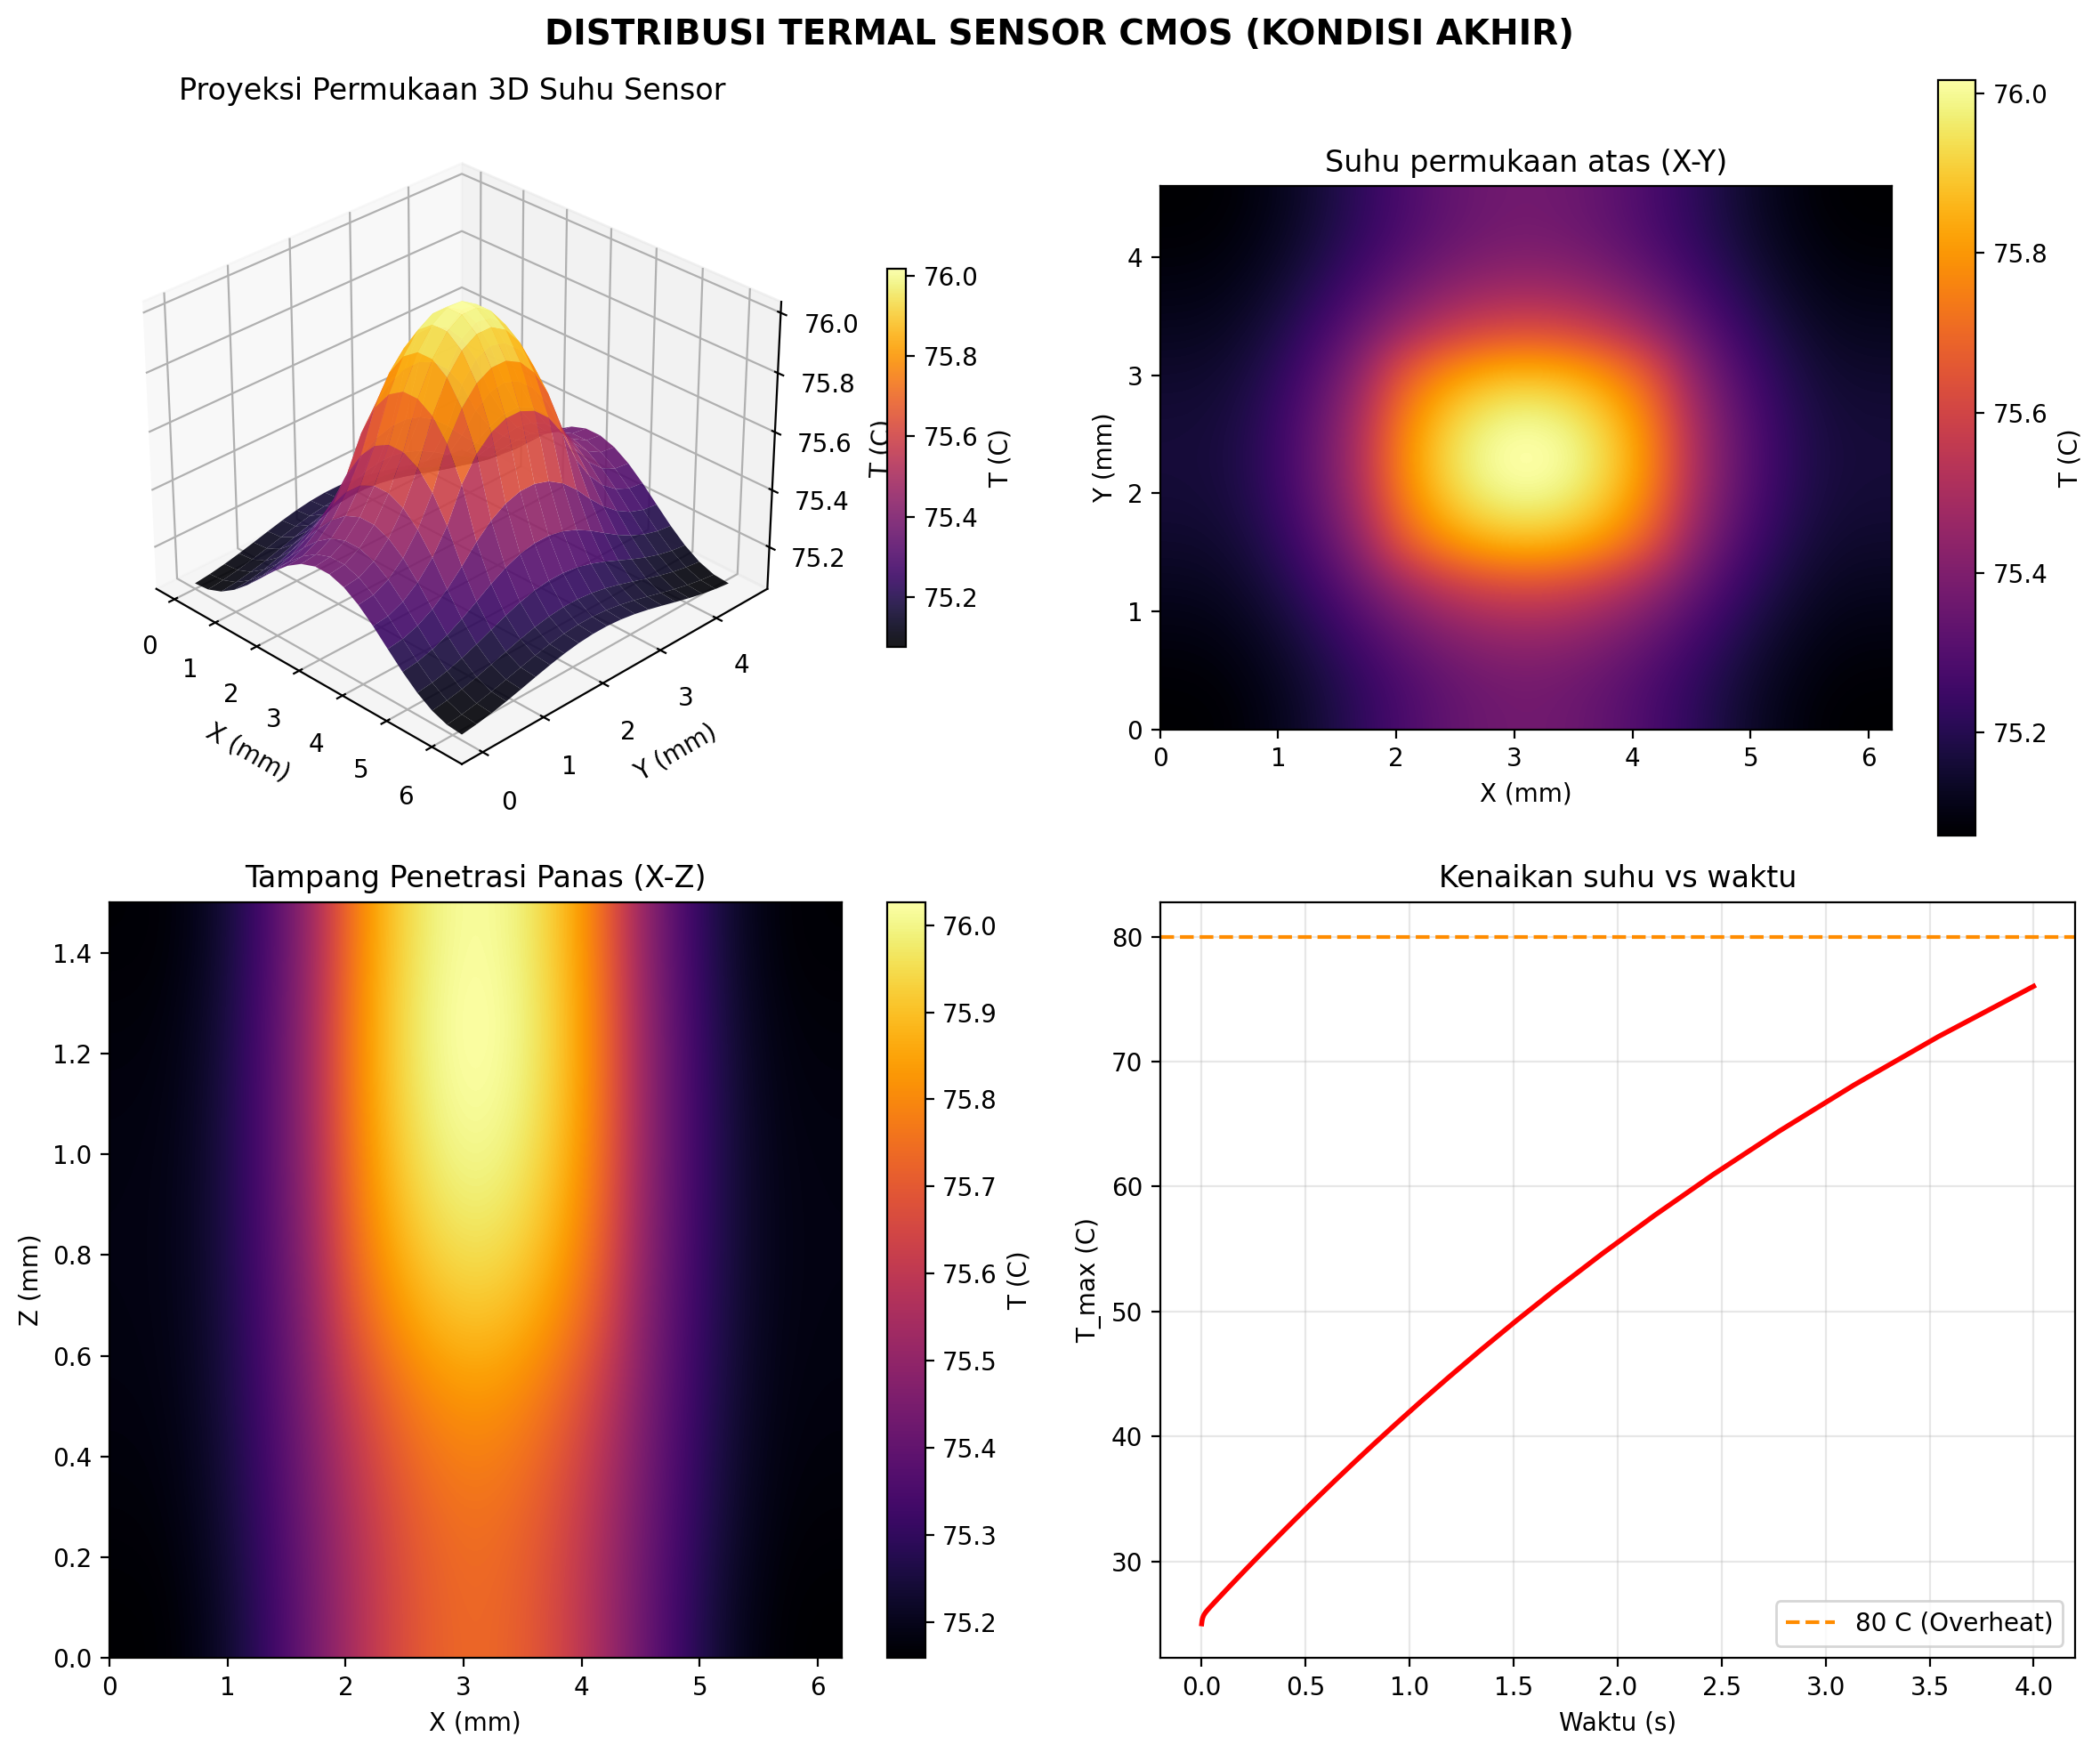
\includegraphics[width=\linewidth]{figures/kasus1.png}
\caption{\textit{Output} program Kasus 1: \textit{dashboard} termal sensor CMOS (peta suhu, penampang X-Z, dan telemetri suhu)}
\label{fig:kasus1}
\end{figure}

% ============================================================
\section{Kasus 2: Distribusi Potensial dan Medan Listrik \textit{Barrel} Lensa dan Rumah Logam (Laplace Silindris)}
% ============================================================

\subsection{Pendahuluan}

\subsubsection{Latar Belakang}
Modul lensa pada kamera \textit{mirrorless} tersusun atas \textit{barrel} lensa, yaitu tabung presisi yang menahan dan menjajarkan elemen-elemen optik. \textit{Barrel} tersebut terpasang di dalam rumah logam (\textit{housing}) yang ditanahkan (\textit{grounded}). Pada sejumlah mekanisme, \textit{barrel} dapat memiliki beda potensial terhadap rumah, baik secara sengaja sebagai elektroda fokus maupun secara tak sengaja akibat akumulasi muatan statik (\textit{electrostatic charging}). Konfigurasi ini secara geometris setara dengan kapasitor koaksial: sebuah konduktor dalam berjari-jari  yang dikelilingi konduktor luar berjari-jari , dengan celah anular (\textit{annular gap}) di antaranya.

Karena \textit{barrel} memiliki panjang berhingga (\textit{finite}), garis medan di kedua ujungnya tidak lagi murni radial sebagaimana pada kapasitor koaksial ideal yang panjangnya tak hingga, melainkan melengkung keluar. Gejala ini dikenal sebagai efek tepi atau \textit{fringing field}, dan tidak dapat dijelaskan oleh rumus koaksial satu dimensi. Untuk memerikan medan secara lengkap, diperlukan penyelesaian dua dimensi pada bidang penampang -. Dalam keadaan bebas muatan ruang (\textit{space charge}), potensial memenuhi persamaan Laplace, yang di sini diselesaikan secara numerik melalui metode beda hingga statik (\textit{Finite-Difference Frequency-Domain}, FDFD).

\subsubsection{Rumusan Masalah}
Permasalahan yang dikaji dapat dirumuskan sebagai berikut: (1) bagaimana distribusi potensial listrik pada celah koaksial antara \textit{barrel} dan rumah; (2) bagaimana arah dan besar medan listrik , termasuk manifestasi efek tepi di ujung \textit{barrel}; serta (3) seberapa akurat solusi numerik FDFD jika ditakar terhadap rumus koaksial analitik pada irisan yang jauh dari ujung.

\subsubsection{Tujuan}
Penelitian ini bertujuan memodelkan celah koaksial \textit{barrel}-rumah secara elektrostatik, menyelesaikan persamaan Laplace koordinat silinder dengan metode FDFD, memvisualisasikan peta potensial beserta vektor arah medan listrik, dan menganalisis efek tepi secara kuantitatif.

\subsection{Teori Dasar}

\subsubsection{Elektrostatika dan Potensial Skalar}
Pada keadaan tunak (\textit{steady-state}), muatan statik tidak bergerak sehingga medan magnet bernilai nol dan seluruh turunan terhadap waktu pada persamaan Maxwell lenyap. Medan listrik elektrostatik bersifat konservatif atau irotasional ($\nabla \times \mathbf{E} = 0$). Sifat ini berimplikasi bahwa kerja yang dilakukan untuk memindahkan muatan tidak bergantung pada lintasan, sehingga medan listrik murni dapat direpresentasikan sebagai gradien dari sebuah fungsi potensial skalar tegangan $V$:

\begin{equation}
\adjustbox{max width=0.95\linewidth}{$\displaystyle \mathbf{E} = -\nabla V$}
\end{equation}

Tanda negatif mengindikasikan bahwa vektor medan listrik selalu menunjuk dari daerah bertegangan tinggi menuju daerah bertegangan rendah (menuruni bukit potensial). Dengan mensubstitusi persamaan di atas ke dalam bentuk diferensial Hukum Gauss untuk medium linear dielektrik seragam ($\nabla \cdot \mathbf{D} = \rho_f$), kita mendapatkan Persamaan Poisson. Dalam absennya muatan bebas murni di udara/vakum celah anular ($\rho_f = 0$), persamaan ini tereduksi menjadi Persamaan Laplace:

\begin{equation}
\adjustbox{max width=0.95\linewidth}{$\displaystyle \nabla^2 V = 0$}
\end{equation}

Secara fisis, Persamaan Laplace bermakna bahwa potensial di titik mana pun merupakan nilai rata-rata persis dari potensial di sekelilingnya (sifat harmonik). Tidak ada puncak atau lembah potensial lokal di wilayah hampa; titik ekstrem selalu berada di batas konduktor (barel dan \textit{housing}).

\subsubsection{Persamaan Laplace Koordinat Silinder}
Mengingat susunan lensa memiliki simetri perputaran sumbu optik ($z$), kita meninjau masalah pada sistem koordinat silinder $(r, \theta, z)$. Karena sistem simetris secara azimutal (potensial tidak bergantung sudut putar $\theta$), turunan $\partial / \partial \theta$ bernilai nol. Penjabaran operator Laplacian $\nabla^2$ dalam koordinat silinder berdimensi dua $r-z$ menjadi:

\begin{equation}
\adjustbox{max width=0.95\linewidth}{$\displaystyle \frac{1}{r}\frac{\partial}{\partial r}\!\left(r\frac{\partial V}{\partial r}\right) + \frac{\partial^2 V}{\partial z^2} = 0 \quad\Rightarrow\quad \frac{\partial^2 V}{\partial r^2} + \frac{1}{r}\frac{\partial V}{\partial r} + \frac{\partial^2 V}{\partial z^2} = 0$}
\end{equation}

Suku eksktra $\frac{1}{r}\frac{\partial V}{\partial r}$ membedakan sistem koordinat silindris dari koordinat Kartesian. Secara geometri, luasan selubung silinder membesar seiring menjauhnya jari-jari $r$, sehingga rapat fluks listrik akan melemah (berkurang). Setelah nilai numerik potensial $V$ direlaksasikan dan didapat, komponen medan listrik vektor diperoleh melalui turunan parsial ruangnya:

\begin{equation}
\adjustbox{max width=0.95\linewidth}{$\displaystyle E_r = -\frac{\partial V}{\partial r}, \qquad E_z = -\frac{\partial V}{\partial z}$}
\end{equation}

\subsubsection{Solusi Koaksial Analitik sebagai Acuan}
Jika kita mengabaikan ujung lensa (menganggap panjang barel tidak terhingga), maka persoalan menjadi 1D radial belaka. Integrasi ganda $\frac{1}{r}\frac{\partial}{\partial r}\left(r\frac{\partial V}{\partial r}\right) = 0$ menghasilkan solusi logaritmik $\ln(r)$. Menerapkan batas tegangan $V(a) = V_0$ pada laras dalam, dan $V(b) = 0$ (\textit{ground}) pada laras luar, menghasilkan solusi teoretis murni (Kapasitor Koaksial Silindris):

\begin{equation}
\adjustbox{max width=0.95\linewidth}{$\displaystyle V(r) = V_0\,\frac{\ln(b/r)}{\ln(b/a)}$}
\end{equation}

Persamaan ini valid secara ketat hanya pada penampang tengah barel. Solusi ini menjadi jangkar kebenaran (\textit{benchmark} analitik) untuk memverifikasi validitas algoritma beda hingga 2D yang kita program.

\subsection{Metodologi}

\subsubsection{Geometri dan Diskritisasi Domain}
Domain komputasi berbentuk persegi panjang pada bidang - dengan jari-jari \textit{barrel}  mm, jari-jari rumah  mm, dan panjang aksial  mm. \textit{Barrel} diberi potensial  V dan sengaja dibuat lebih pendek daripada domain agar efek tepi terpapar di kedua ujungnya. Domain didiskritisasi memakai kisi (\textit{grid}) seragam berukuran  titik, dengan langkah ruang  dan  yang seragam.

\subsubsection{Stensil Beda Hingga Konservatif}
Persamaan Laplace didiskritisasi memakai stensil konservatif (\textit{conservative/flux-preserving stencil}) yang mengevaluasi koefisien radial pada muka antar-sel di posisi setengah-indeks , sehingga fluks listrik yang melintasi tiap muka kendali terjaga secara diskret:

\begin{equation}
\adjustbox{max width=0.95\linewidth}{$\displaystyle \frac{V_{i+1,j}-2V_{i,j}+V_{i-1,j}}{\Delta r^2} + \frac{1}{r_i}\frac{V_{i+1,j}-V_{i-1,j}}{2\,\Delta r} + \frac{V_{i,j+1}-2V_{i,j}+V_{i,j-1}}{\Delta z^2} = 0$}
\end{equation}
Pada sumbu  diberlakukan syarat regularitas (\textit{regularity condition}) berupa  untuk menghindari singularitas suku , sedangkan permukaan \textit{barrel}, rumah, dan batas domain memakai syarat Dirichlet. Seluruh titik kisi dirakit menjadi sistem persamaan linear \textit{sparse} . Sistem ini diselesaikan secara langsung (\textit{direct solver}) melalui dekomposisi LU \textit{sparse} (\textit{SuperLU}) yang dipanggil melalui fungsi spsolve, lalu komponen medan listrik dihitung dengan skema beda tengah (\textit{central difference}).

\subsubsection{Algoritma dan Akselerasi Komputasi}
Perakitan matriks (\textit{matrix assembly}) yang memuat banyak elemen titik batas dapat berjalan lambat jika dieksekusi dengan perulangan standar Python, terutama ketika struktur matriks perlu diperbarui untuk setiap simulasi gerakan aktuator lensa. Untuk mengoptimalkan waktu komputasi, fungsi pembentukan elemen dieksekusi bersama fungsi \textit{Just-In-Time} (JIT) melalui paket modul \textit{Numba} (\texttt{@njit}). \textit{Numba} mereduksi latensi interpretasi operasional bawaan Python menjadi instruksi level perangkat keras (\textit{machine code}). Matriks jarang (\textit{sparse matrix}) dimensi besar ($A \cdot x = b$) ini kemudian dikomputasi menggunakan subrutin dekomposisi \textit{LU} (SuperLU) milik SciPy. Eksekusi JIT \textit{Numba} dan metode pencari invers langsung \textit{SuperLU} mempercepat iterasi penyelesaian secara keseluruhan tanpa perlu perhitungan metode tebak-ralat iteratif.

\subsection{Hasil dan Pembahasan}

Berdasarkan komputasi pada Gambar \ref{fig:kasus2}, distribusi fluks tergambar melalui gradien pemetaan nilai skalar beda potensial ($V$) dan panah vektor medan listrik ($E$). Di rentang silinder tengah barel konduktor, garis medan terdistribusi merata dengan sudut tegak lurus terhadap arah pelat. Arah orientasi panah melukiskan lintasan elektron fiktif menuju luar (area ground potensial rendah).

Pada rentang posisi ujung barel eksterior, tampak garis medan listrik melengkung (deviasi radial asimetris). Kelengkungan medan ekuipotensial eksterior (\textit{fringing field}) terjadi akibat fakta bahwa pelat konduktor (barel lensa kamera) bukan bersifat memanjang tak terhingga seperti pada hukum Gauss asimtotik. Fenomena fisis dua dimensi ini dapat disimulasikan menggunakan matriks \textit{sparse} stensil batas fisis, yang merangkum variasi nilai ruang di setiap piksel untuk merekam "kebocoran" arah orientasi tanpa batasan aproksimasi komputasi yang rumit.

Untuk validasi, ditunjukkan profil perbandingan gradien skalar lintang batas $V(r)$ tengah silinder. Perbandingan garis data komputasi ekuivalen (titik dot) dan kurva acuan logaritma aproksimasi Gauss analitik (putus-putus) menunjukkan akurasi resolusi simulasi numerikal dalam metode diskritisasi yang cukup presisi, mencatatkan defisiasi toleransi \textit{error} minor $\approx 2,08\%$. Faktor persentase kecil tersebut berasal dari limitasi panjang matriks kisi ruang ($\Delta r$) serta pelebaran minor dari deviasi (\textit{fringing}) ke arah sentral geometri. Hal ini membuktikan kemampuan FDFD metode konservatif bagi pemodelan elektrostatika tabung ruang nyata.

\begin{figure}[H]
\centering
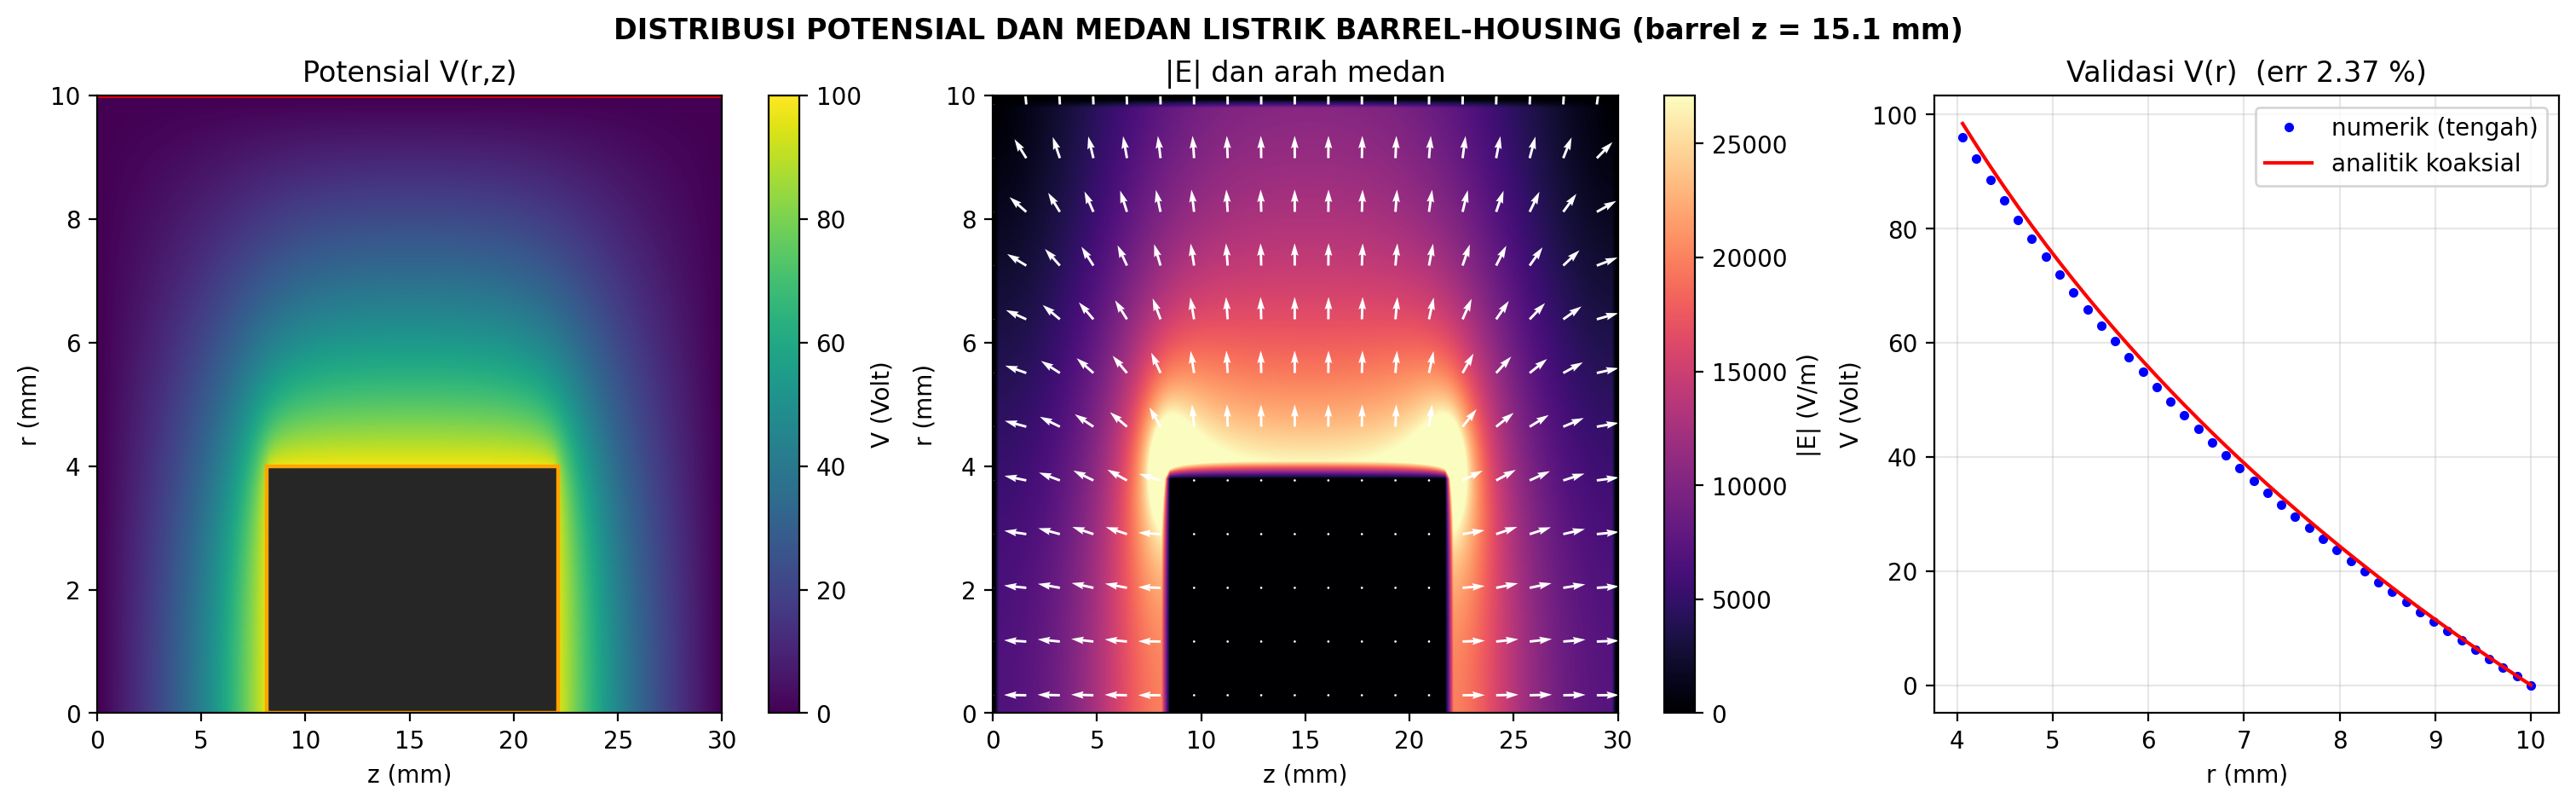
\includegraphics[width=\linewidth]{figures/kasus2.png}
\caption{\textit{Output} program Kasus 2: elektrostatik \textit{barrel}-\textit{housing} (potensial, besar dan arah medan, serta validasi koaksial)}
\label{fig:kasus2}
\end{figure}

% ============================================================
\section{Kasus 3: Distribusi Medan Listrik pada \textit{Dome Port} Dielektrik dalam Medan Seragam (Volume Hingga)}
% ============================================================

\subsection{Pendahuluan}

\subsubsection{Latar Belakang}
Pada kamera bawah air (\textit{underwater housing}), di depan modul lensa dipasang \textit{dome port}, yaitu kubah transparan berbahan dielektrik seperti akrilik atau kaca optik yang berfungsi mempertahankan sudut pandang lensa sekaligus meminimalkan distorsi refraksi pada antarmuka air-udara. Ketika dome berada dalam medan listrik eksternal, misalnya akibat muatan statik terlarut di lingkungan air, material dome mengalami polarisasi (\textit{polarization}). Polarisasi ini membangkitkan muatan terikat (\textit{bound charge}) pada permukaan dome, yang selanjutnya mengubah sebaran medan, baik di dalam maupun di sekitar kubah.

Oleh karena tidak terdapat muatan bebas pada material, potensial tetap memenuhi persamaan Laplace, tetapi dengan lompatan permitivitas (\textit{permittivity jump}) pada antarmuka dome. Penanganan lompatan ini menuntut formulasi yang menjaga kontinuitas komponen normal medan perpindahan listrik (\textit{displacement field}) . Geometri bola tidak memiliki solusi analitik tertutup untuk konfigurasi sembarang, sehingga persoalan diselesaikan secara numerik dengan metode volume hingga (\textit{finite volume} \textit{method}, FVM).

\subsubsection{Rumusan Masalah}
Permasalahan yang dikaji: (1) bagaimana distribusi medan listrik di dalam dan di sekitar dome dielektrik yang ditempatkan dalam medan seragam; (2) bagaimana perilaku garis medan saat melintasi antarmuka dielektrik; serta (3) seberapa besar atenuasi medan di bagian dalam dome dibandingkan dengan prediksi analitik bola dielektrik klasik.

\subsubsection{Tujuan}
Penelitian bertujuan menyelesaikan persamaan Laplace koordinat bola dengan syarat batas dielektrik menggunakan metode volume hingga, memvisualisasikan besar dan arah medan listrik, dan memvalidasi medan interior dome terhadap hasil klasik bola dielektrik dalam medan seragam.

\subsection{Teori Dasar}

\subsubsection{Elektrostatika Medium Dielektrik dan Polarisasi}
Berbeda dengan bahan konduktor yang membiarkan muatan bergerak bebas ke permukaan, material dielektrik seperti akrilik (kaca) pada lensa penutup bawah air terbuat dari atom-atom yang menahan erat elektronnya. Ketika kubah diletakkan di tengah medan listrik eksternal $\mathbf{E}_{0}$, atom-atom material merespon dengan memelarkan posisi awan elektron relatif terhadap inti (polarisasi). Ini menciptakan momen dipol terinduksi berskala makroskopik yang direpresentasikan dengan rapat polarisasi $\mathbf{P}$.

Kehadiran polarisasi membangkitkan muatan-muatan terikat (\textit{bound charge}) tepat di permukaan batas antar-muka medium. Untuk mengakomodasi hal ini tanpa repot melacak sebaran spesifik $\rho_{bound}$, Maxwell memperkenalkan vektor perpindahan listrik $\mathbf{D} = \varepsilon_0 \mathbf{E} + \mathbf{P} = \varepsilon \mathbf{E}$. Di kawasan tanpa muatan bebas, divergensinya harus nol. Dengan mensubstitusi $\mathbf{E} = -\nabla V$, diperoleh hukum Gauss Dielektrik:

\begin{equation}
\adjustbox{max width=0.95\linewidth}{$\displaystyle \nabla\cdot\left(\varepsilon(\mathbf{r})\,\nabla V\right) = 0$}
\end{equation}

Perhatikan bahwa konstanta $\varepsilon$ tak dapat ditarik keluar dari operator divergensi $\nabla$ karena ia bernilai spesifik sebagai fungsi posisi $\mathbf{r}$. Nilai ini akan mengalami lompatan (diskontinuitas atau permittivity jump) eksak pada tepian cangkang dari permitivitas udara ($\varepsilon_0$) menjadi permitivitas akrilik ($\varepsilon_r \varepsilon_0$).

Syarat batas diskontinuitas normal secara matematis menyatakan fluks $\mathbf{D}_{\perp}$ harus kontinu melintasi dinding (tidak ada muatan bebas terjebak), yang berimplikasi pada pembiasan atau tekukan mendadak lintasan fluks medan saat masuk:
\begin{equation}
\adjustbox{max width=0.95\linewidth}{$\displaystyle \left( \varepsilon_{\text{air}}\frac{\partial V}{\partial n} \right)_{\text{keluar}} = \left( \varepsilon_{\text{kaca}}\frac{\partial V}{\partial n} \right)_{\text{masuk}}$}
\end{equation}
Untuk menangani kondisi pelik diskontinuitas batas secara elegan tanpa tebakan fungsi aneh, teknik diskritisasi Metode Volume Hingga (FVM) digunakan.

\subsubsection{Persamaan Laplace Koordinat Bola}
Model setengah bola menuntut \textit{grid} komputasi koordinat polar silindris $(r, \theta)$. Operator nabla disesuaikan sehingga persamaan konservatif dielektrik mengambil wujud:
\begin{equation}
\adjustbox{max width=0.95\linewidth}{$\displaystyle \frac{1}{r^2}\frac{\partial}{\partial r}\left(r^2 \varepsilon \frac{\partial V}{\partial r}\right) + \frac{1}{r^2 \sin\theta}\frac{\partial}{\partial \theta}\left(\varepsilon \sin\theta \frac{\partial V}{\partial \theta}\right) = 0$}
\end{equation}
Setiap turunan di atas mengekspresikan total divergensi rapat luasan diferensial permukaan dari setiap kubus parsial \textit{grid} bola.

\subsubsection{Solusi Klasik Bola Dielektrik}
Bila asumsinya bola pejal seragam dengan radius $a$ direndam di dalam medan homogen $E_0$ searah sumbu z, penyelesaian teoritik kalkulus ekspansi harmonik bola (deret Legendre) mampu mendemonstrasikan bahwa medan internal yang timbul harus selalu bervektor seragam, paralel searah $E_0$, dan lebih lemah (tereduksi akibat tarikan kebalikan dari $\mathbf{P}$). Besaran teoritis pelemahan tegangan tersebut (Depolarisasi) eksak bernilai:
\begin{equation}
\adjustbox{max width=0.95\linewidth}{$\displaystyle E_{\mathrm{dalam}} = \frac{3}{\varepsilon_r + 2}\,E_0$}
\end{equation}
Rumus analitik $E_{\mathrm{dalam}}$ inilah yang menjadi nilai acuan kebenaran absolut untuk mengonfirmasi kinerja simulasi FVM 2D kita, dengan mengharapkan tingkat kesalahan kurang dari $5\%$.

\subsection{Metodologi}

\subsubsection{Diskritisasi Volume Hingga (FVM)}
Metode Volume Hingga mengevaluasi hukum konservasi bukan pada simpul titik, melainkan mengintegrasikan divergensi ke seluas seluruh volume kubus per-sel (menggunakan Teorema Divergensi Gauss $\iiint \nabla \cdot (\dots) d\tau = \iint (\dots) \cdot dA $).
Ini mereduksi persoalan menjadi perhitungan murni fluks masuk dari sel tetangga, yang disederhanakan sebagai:
\begin{equation}
\adjustbox{max width=0.95\linewidth}{$\displaystyle \sum_{\text{muka}} \left(\varepsilon \cdot A_{\text{muka}} \cdot \frac{\partial V}{\partial n}\right) = 0$}
\end{equation}
Otomatis, di daerah patahan batas $\varepsilon_r$, metode ini langsung mengambil jembatan nilai interpolasi rata-rata harmonik (interpolasi permitivitas silang muka), sehingga memastikan persyaratan lompatan syarat batas Gauss dipatuhi tanpa perlu pengkodisian matriks terpisah. Pada daerah kutub singularitas ($\theta = 0, r=0$), muka luasan $A_{\text{muka}} = 0$ sehingga suku pecah singular terbuang dengan sendirinya, sebuah sihir matematis elegan dari FVM.

\subsubsection{Algoritma dan Akselerasi Komputasi}
Perakitan dimensi stensil koefisien rasio sel dalam sistem matriks bola untuk \textit{Finite Volume Method} (FVM) menuntut beban siklus eksekusi yang tinggi jika dilakukan hanya melalui fitur sintaks iterasi Python murni. Untuk mengakselerasi komputasi matriks \textit{grid} tersebut, diimplementasikan paket optimasi dekorator kompilasi \textit{Just-In-Time} (JIT) \texttt{@njit} dari pustaka \textit{Numba}. \textit{Numba} mentranslasi bahasa operasi \textit{array} Python ke dalam komputasi level sistem untuk menekan \textit{overhead} pada \textit{loop} iterasi. Matriks linear $M \cdot x = b$ hasil FVM dialokasikan ruangnya ke format kordinat memori data 5-diagonal tipis \textit{Coordinate Format} (COO), sehingga memudahkan fungsi pustaka bawaan linier \textit{SciPy} untuk mencari balikan (invers) operasi perhitungan dengan tepat dan efisien. Penambahan JIT \textit{Numba} mempercepat siklus simulasi hingga pergerakan 20 tahapan medan luaran optik dielektrik dapat tersaji dalam kalkulasi sub-detik komputasional.

\subsection{Hasil dan Pembahasan}

Visualisasi kontur pada Gambar \ref{fig:kasus3} (Kiri) merepresentasikan amplitudo besar medan listrik $|\mathbf{E}|$. Secara eksterior (luar), arah penyebaran fluks merambat dalam bentuk gelombang konstan linear dan merata ($E_0$). Mendekati perbatasan batas (\textit{boundary}) dengan cangkang \textit{dome port} dielektrik (ditandai oleh garis batas merah putus-putus), arah perambatan vektor orientasi refraksi medan panah $\mathbf{E}$ membelok ke arah radial. Pembengkokan garis gaya medan tersebut membuktikan keberadaan intervensi orientasi (induksi polarisasi molekuler) karena perubahan permitivitas diskontinu antarmuka antara area hampa ke akrilik dielektrik. Rentang area interior bola juga ditandai dengan perubahan kontur gradien warna biru pekat. Perbedaan tajam skalar warna ini mendemonstrasikan fenomena fisika efektivitas absorpsi redaman (\textit{depolarization} tameng) akibat susunan polarisasi induksi yang terjadi secara spasial dalam material dielektrik terkait.

Berdasarkan perbandingan irisan medan pada \texttt{E_z} sumbu sentral simetris (Gambar \ref{fig:kasus3} Kanan), dapat dilihat karakteristik ekuivalen pada perambatan medan dielektrik yang lebih homogen. Titik-titik luaran komputasi membentuk lereng horizontal lurus (konstan mendatar) murni selama merambat sejauh jarak rentang limit radius interior geometri bola $R$. Penurunan rata-rata (atenuasi) pada internal \textit{dome} ditaksir pada nilai besaran $\approx 540.0\text{ V/m}$. Nilai diskritisasi batas FVM numerik tersebut mendekati garis batas referensi kalkulasi rasio teoretik (Hukum Gauss murni) di besaran nilai ukur sebesar $\approx 555.6\text{ V/m}$. Presisi yang memuat perbedaan margin \textit{error} hanya dengan porsi toleransi nilai selisih $< 2,8\%$ membuktikan kemampuan metode algoritma komputasi interpolasi batas harmonik \textit{FVM cell-centered} mengaproksimasi lompatan fasa gelombang radial diskontinu di batas geometri lengkung (yang mana terkadang menghasilkan fluktuasi lokal kecil \textit{aliasing peak} atau \textit{spike} pada batas resolusi celah \textit{grid} komputasi).

\begin{figure}[H]
\centering
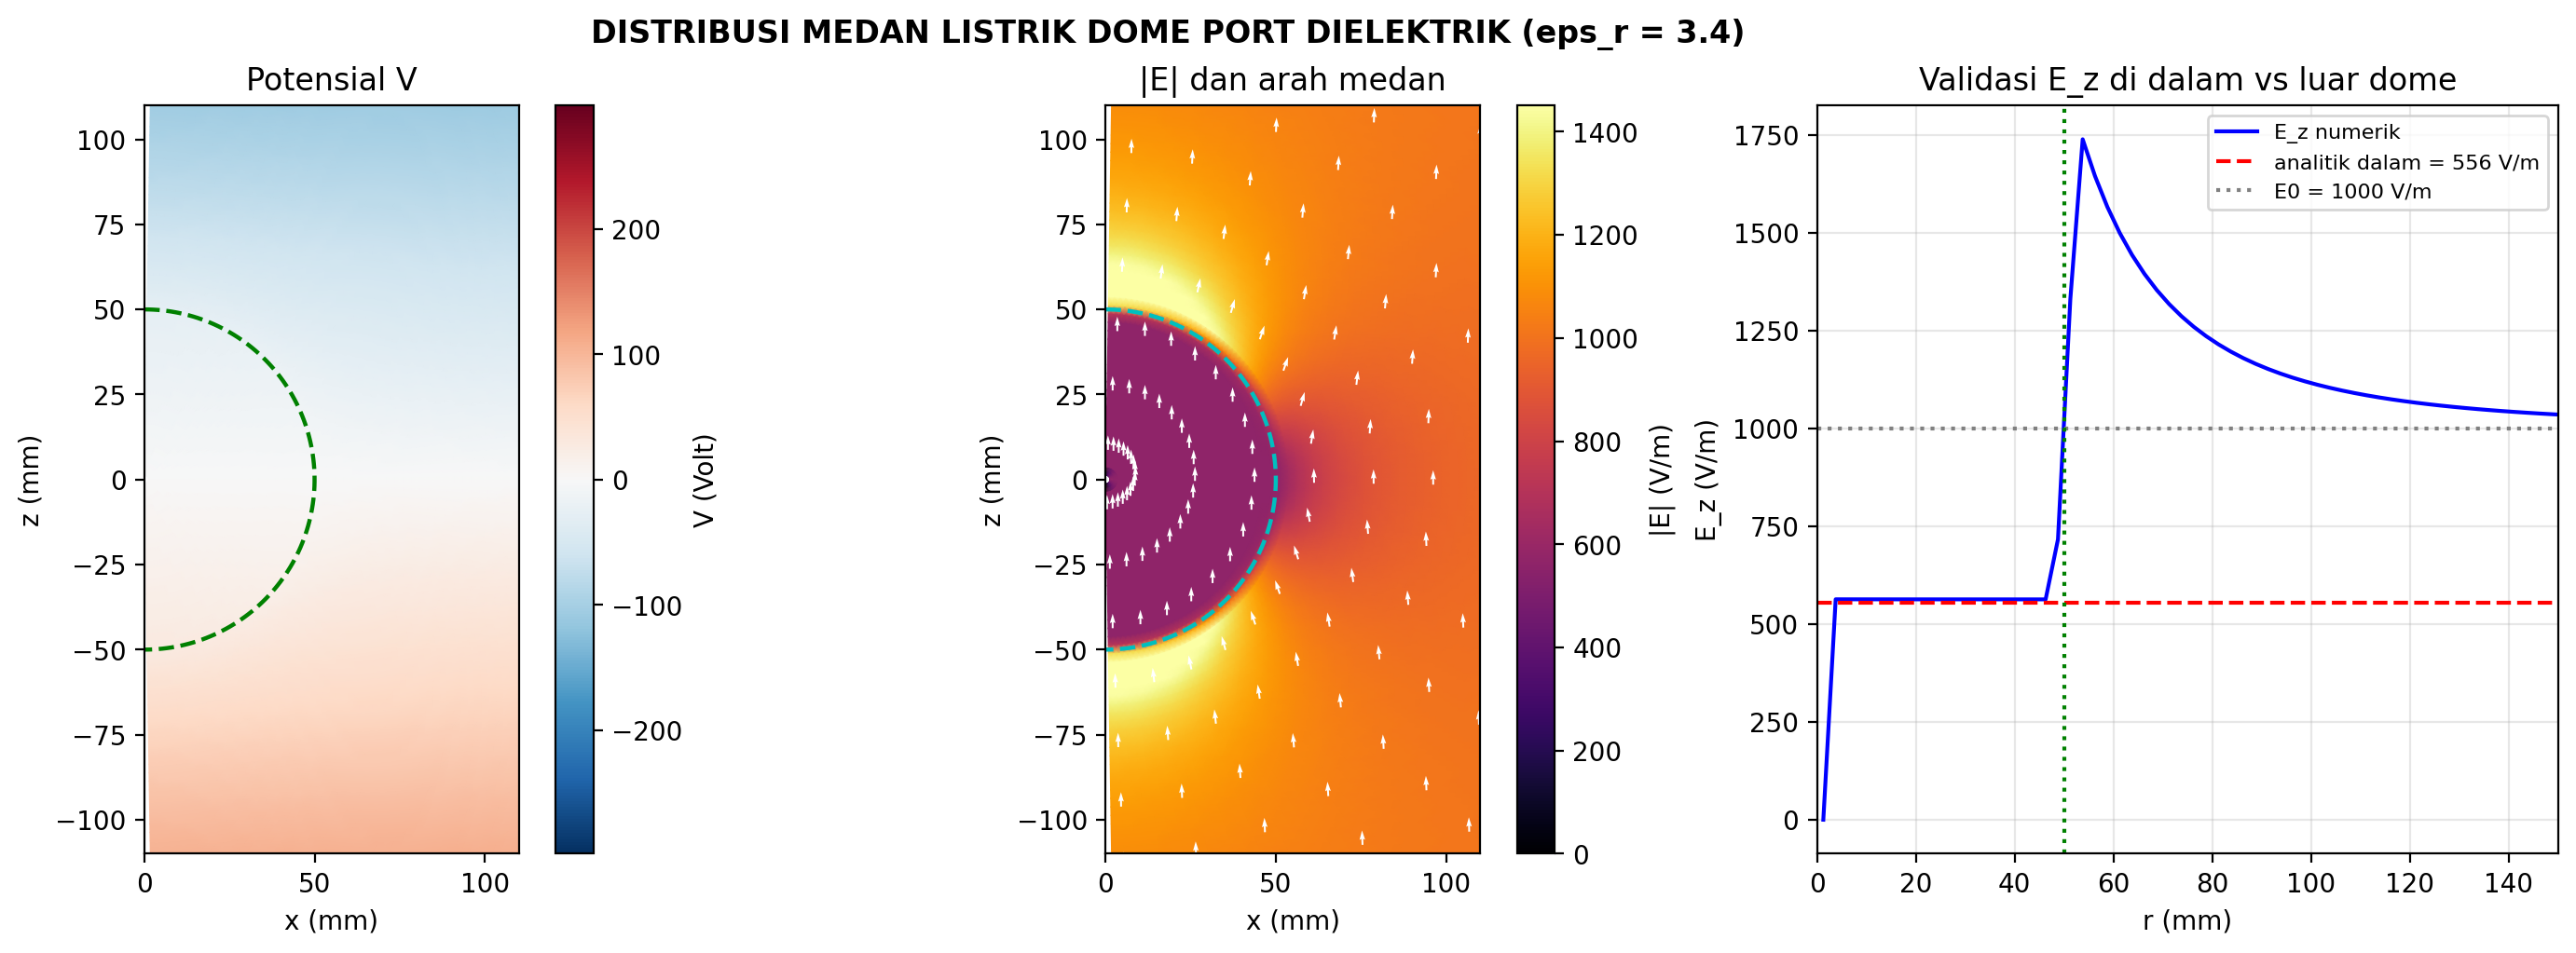
\includegraphics[width=\linewidth]{figures/kasus3.png}
\caption{\textit{Output} program Kasus 3: \textit{dome port} dielektrik (potensial, besar dan arah medan, serta validasi medan dalam)}
\label{fig:kasus3}
\end{figure}

% ============================================================
\section{Kasus 4: Distribusi Medan Magnet Aktuator Voice Coil Motor (Magnetostatik Silindris)}
% ============================================================

\subsection{Pendahuluan}

\subsubsection{Latar Belakang}
Voice Coil Motor (VCM) merupakan aktuator elektromagnetik yang banyak digunakan pada sistem autofokus kamera digital modern. Komponen ini berfungsi mengubah energi listrik menjadi gerakan translasi linier yang digunakan untuk menggeser posisi lensa sehingga fokus dapat diatur secara otomatis. Dibandingkan mekanisme aktuator lainnya, VCM memiliki keunggulan berupa ukuran yang kecil, respons yang cepat, konsumsi daya yang rendah, serta kemampuan menghasilkan perpindahan dengan presisi tinggi. Oleh karena itu, teknologi ini banyak diterapkan pada kamera telepon pintar, kamera digital, serta berbagai sistem optik miniatur. kerja VCM didasarkan pada gaya Lorentz yang timbul akibat interaksi antara arus listrik yang mengalir pada kumparan dengan medan magnet di sekitarnya. Ketika arus diberikan pada kumparan, medan magnet yang terbentuk akan berinteraksi dengan medan magnet permanen sehingga menghasilkan gaya elektromagnetik. Besarnya gaya yang dihasilkan sangat dipengaruhi oleh distribusi medan magnet di dalam aktuator. Oleh sebab itu, pemahaman mengenai distribusi medan magnet menjadi faktor penting dalam proses perancangan dan optimasi kinerja VCM. kajian magnetostatika, distribusi medan magnet dapat dihitung menggunakan pendekatan potensial vektor magnetik. Berbeda dengan medan listrik yang sering dianalisis melalui potensial skalar, medan magnet lebih mudah ditangani menggunakan potensial vektor karena memenuhi sifat divergensi nol. Karena geometri VCM berbentuk silindris dan melibatkan distribusi sumber yang terlokalisasi pada daerah kumparan, solusi analitik hanya tersedia untuk konfigurasi yang sangat sederhana. Pada konfigurasi yang lebih realistis, distribusi medan magnet harus diperoleh secara numerik. Salah satu metode yang banyak digunakan adalah metode volume hingga (\textit{Finite Volume} \textit{Method} atau FVM), yaitu metode numerik yang mempertahankan sifat konservatif dari persamaan diferensial dan mampu menangani geometri yang kompleks dengan baik. Pada penelitian ini, distribusi potensial vektor magnetik dan medan magnet pada aktuator VCM autofokus silindris dianalisis menggunakan metode volume hingga. Hasil simulasi divisualisasikan dalam bentuk peta distribusi medan magnet dan dibandingkan dengan teori solenoida untuk mengevaluasi ketepatan metode numerik yang digunakan.

\subsubsection{Rumusan Masalah}
\begin{enumerate}[itemsep=1pt,topsep=2pt]
\item Bagaimana distribusi potensial vektor magnetik pada aktuator Voice Coil Motor (VCM) autofokus silindris yang dialiri arus listrik.
\item Bagaimana distribusi medan magnet yang dihasilkan oleh kumparan pada daerah di dalam dan di sekitar aktuator.
\item Bagaimana karakteristik profil medan magnet pada sumbu utama aktuator.
\item Seberapa baik metode volume hingga mampu merepresentasikan distribusi medan magnet dibandingkan dengan teori magnetostatika klasik.
\end{enumerate}

\subsubsection{Tujuan}
\begin{enumerate}[itemsep=1pt,topsep=2pt]
\item Menyelesaikan Persamaan Poisson magnetostatik menggunakan metode volume hingga pada geometri silindris.
\item Memvisualisasikan distribusi potensial vektor magnetik dan medan magnet yang dihasilkan oleh kumparan VCM.
\item Mengkaji karakteristik medan magnet yang berperan dalam pembangkitan gaya elektromagnetik pada sistem autofokus.
\item Memvalidasi hasil numerik terhadap teori solenoida sebagai acuan analitik.
\end{enumerate}

\subsection{Teori Dasar}

\subsection{Teori Dasar}

\subsubsection{Magnetostatika dan Potensial Vektor Magnetik}
Magnetostatika merupakan cabang elektromagnetika yang mempelajari medan magnet tunak yang dihasilkan oleh distribusi arus konstan (tidak berubah terhadap waktu, $\partial/\partial t = 0$). Karena medan magnet selalu membentuk \textit{loop} tertutup (tidak ada monopol magnetik), divergensi dari fluks magnetik harus nol $\nabla \cdot \mathbf{B} = 0$. Secara matematis, sifat eksak divergen nol ini memungkinkan kita mendefinisikan medan magnet $\mathbf{B}$ sebagai ikal (\textit{curl}) dari sebuah medan vektor yang disebut potensial vektor magnetik $\mathbf{A}$:

\begin{equation}
\adjustbox{max width=0.95\linewidth}{$\displaystyle \mathbf{B} = \nabla \times \mathbf{A}$}
\end{equation}

Sesuai dengan Hukum Ampere $\nabla \times \mathbf{B} = \mu \mathbf{J}$, jika kita mensubstitusi persamaan vektor di atas, kita mendapatkan:
\begin{equation}
\adjustbox{max width=0.95\linewidth}{$\displaystyle \nabla \times (\nabla \times \mathbf{A}) = \mu \mathbf{J} \quad\Rightarrow\quad \nabla(\nabla \cdot \mathbf{A}) - \nabla^2 \mathbf{A} = \mu \mathbf{J}$}
\end{equation}
Dengan bebas menerapkan \textit{Coulomb Gauge} ($\nabla \cdot \mathbf{A} = 0$), persamaan rumit ini merosot (tereduksi) menjadi bentuk Persamaan Poisson vektor yang elegan dan lebih mudah dipecahkan oleh komputer:

\begin{equation}
\adjustbox{max width=0.95\linewidth}{$\displaystyle \nabla^2 \mathbf{A} = -\mu\,\mathbf{J}$}
\end{equation}

Makna fisis dari $\mathbf{A}$ menyerupai fungsi arus (stream \textit{function}). Garis kontur yang bernilai konstan $A =$ konstan mewakili lintasan fluks $\mathbf{B}$ itu sendiri. Sumber pembentuk $\mathbf{A}$ adalah rapat arus listrik vektor $\mathbf{J}$ yang beredar dalam kabel kumparan VCM.

\subsubsection{Persamaan Poisson pada Koordinat Silinder}
Kumparan Voice Coil Motor (VCM) dililit menyerupai tabung donat. Karenanya, masalah ditinjau pada koordinat silindris $(r, \phi, z)$. Rapat arus $\mathbf{J}$ hanya mengalir memutar mengikuti keliling kawat azimutal searah komponen $\hat{\phi}$ sehingga $J_r = J_z = 0$. Akibatnya, komponen potensial vektor yang bangkit juga murni azimutal $\mathbf{A} = A_\phi \hat{\phi}$. Ekspansi Laplacian vektor untuk $A_\phi$ menyisakan suku singular pada sumbu $r$:

\begin{equation}
\adjustbox{max width=0.95\linewidth}{$\displaystyle \frac{\partial^2 A_\phi}{\partial r^2} + \frac{1}{r}\frac{\partial A_\phi}{\partial r} - \frac{A_\phi}{r^2} + \frac{\partial^2 A_\phi}{\partial z^2} = -\mu J_\phi$}
\end{equation}
Penambahan suku negatif $-A_\phi / r^2$ secara matematis memaksa nilai potensial harus bernilai persis nol di pusat $r = 0$, mencegah solusi dari divergensi hingga meledak ke tak terhingga.

\subsubsection{Perhitungan Medan Magnet $\mathbf{B}$}
Setelah nilai $A_\phi$ dipecahkan secara numerik di setiap \textit{grid}, nilai fisis medan listrik radial dan aksial langsung diturunkan dari definisi putarannya $\mathbf{B} = \nabla \times \mathbf{A}$:

\begin{equation}
\adjustbox{max width=0.95\linewidth}{$\displaystyle B_r = -\frac{\partial A_\phi}{\partial z}, \qquad B_z = \frac{1}{r}\frac{\partial\left(r A_\phi\right)}{\partial r}$}
\end{equation}
Besarnya total medan magnet skalar diturunkan dari penjumlahan vektor phytagoras $|\mathbf{B}| = \sqrt{B_r^2 + B_z^2}$.

\subsubsection{Solusi Klasik Solenoida sebagai Acuan}
Sistem kumparan panjang ekuivalen secara asimtotik dengan solenoida. Di bagian tengah rongga inti (menjauh dari tepian), medan magnet memadat menjadi satu arah sumbu-z ($B_z$) bernilai konstan, tak bergantung pada $r$. Persamaan klasik ini dirumuskan sebagai:
\begin{equation}
\adjustbox{max width=0.95\linewidth}{$\displaystyle B = \mu_0 n I$}
\end{equation}
Dengan $n$ adalah kerapatan lilitan (lilitan per meter). Nilai ini dipakai sebagai pembanding teoretis yang menguji keakuratan matriks yang dirakit FVM.

\subsection{Metodologi}

\subsubsection{Diskritisasi Volume Hingga (FVM)}
Persamaan Poisson $A_\phi$ diferensial dikonversi ke bentuk kekekalan fluks makroskopik di atas jaring sel 2D $(r, z)$ berukuran sel $\Delta r \times \Delta z$. Teorema Stokes diberlakukan di sekeliling wilayah irisan koil VCM. Persamaan volume hingga merekam fluks difusif dari ke-empat dinding sel: Utara, Selatan, Barat, dan Timur, diikat oleh suku pusaran $-a_p / r_i^2$:
\begin{equation}
\adjustbox{max width=0.95\linewidth}{$\displaystyle a_p = -\left(a_e + a_w + a_n + a_s\right) - \frac{\text{Volume}_i}{r_i^{\,2}}$}
\end{equation}
Pada pusat laras (sumbu simetri $r=0$), nilai $A_\phi$ di-nol-kan secara eksplisit (\textit{Dirichlet Boundary}).

\subsubsection{Algoritma dan Akselerasi Komputasi}
Pencarian solusi distribusi medan magnet dengan metode iteratif konvensional seperti \textit{Successive Over-Relaxation} (SOR) dapat memakan waktu komputasi yang lama. Sebagai alternatif yang lebih efisien, algoritma pada simulasi ini langsung merakit persamaan-persamaan beda hingga ke dalam satu matriks koefisien besar. Fungsi perakitan matriks ini diakselerasi menggunakan kompiler JIT dari \textit{Numba} melalui dekorator \texttt{@njit}. \textit{Numba} membantu mempercepat proses pengisian elemen matriks ke format koordinat (\textit{Coordinate Format}/COO) di dalam perulangan bersarang. Dengan menggunakan \textit{Numba}, waktu komputasi untuk menyusun matriks dapat direduksi dari hitungan menit (jika menggunakan Python standar) menjadi di bawah 0,1 detik. Matriks \textit{sparse} yang terbentuk kemudian diselesaikan menggunakan pemecah matriks linear dari SciPy (\texttt{scipy.sparse.linalg.spsolve}) untuk mendapatkan distribusi potensial vektor yang akan diplot.

\subsection{Hasil dan Pembahasan}

Berdasarkan distribusi kuat medan magnet $|\mathbf{B}|$ pada Gambar \ref{fig:kasus4} (Kiri), intensitas medan tertinggi (warna kuning) berada pada area kumparan kawat silindris di $r > 0$. Hal ini sesuai dengan konsep fisika dasar, karena pada area tersebut terdapat rapat arus ($\mu J_\phi$) yang merupakan sumber medan. Konsentrasi medan pada titik kawat menunjukkan letak induksi magnetik maksimum dengan nilai mencapai $B_{\mathrm{maks}} = 2{,}90 \times 10^{-4}$ Tesla.

Arah vektor medan yang ditunjukkan oleh panah putih juga sesuai dengan Kaidah Tangan Kanan. Garis fluks mengalir ke atas di bagian dalam tabung (sepanjang sumbu $z$), berbelok ke arah luar di ujung atas kumparan, dan mengalir kembali ke bawah melewati sisi luar kumparan untuk membentuk siklus tertutup. Kurva putaran tertutup ini merupakan visualisasi dari sifat divergensi nol atau \textit{solenoidal} pada medan magnet ($\nabla \cdot \mathbf{B} = 0$), yang berarti garis gaya magnet tidak memiliki titik awal atau akhir yang jelas (tidak adanya monopol magnet).

Pada panel kanan, grafik nilai medan magnet di sepanjang sumbu utama ($B_z$) terhadap posisi aksial ($z$) menunjukkan bahwa medan magnet terkuat berada di titik tengah kumparan. Kekuatan medan ini kemudian berkurang secara perlahan saat mendekati pinggiran laras aktuator. Karakteristik pelemahan medan ini sejalan dengan profil medan solenoida hingga pada bagian ujungnya. Titik-titik merah (hasil numerik) juga berhimpitan dengan garis putus-putus acuan analitik yang bernilai $\approx 2.51 \times 10^{-4}$ T (dari batas $\mu_0 n I$). Kesesuaian hasil antara komputasi FVM dan analitik membuktikan bahwa algoritma yang digunakan telah bekerja secara akurat.

\begin{figure}[H]
\centering
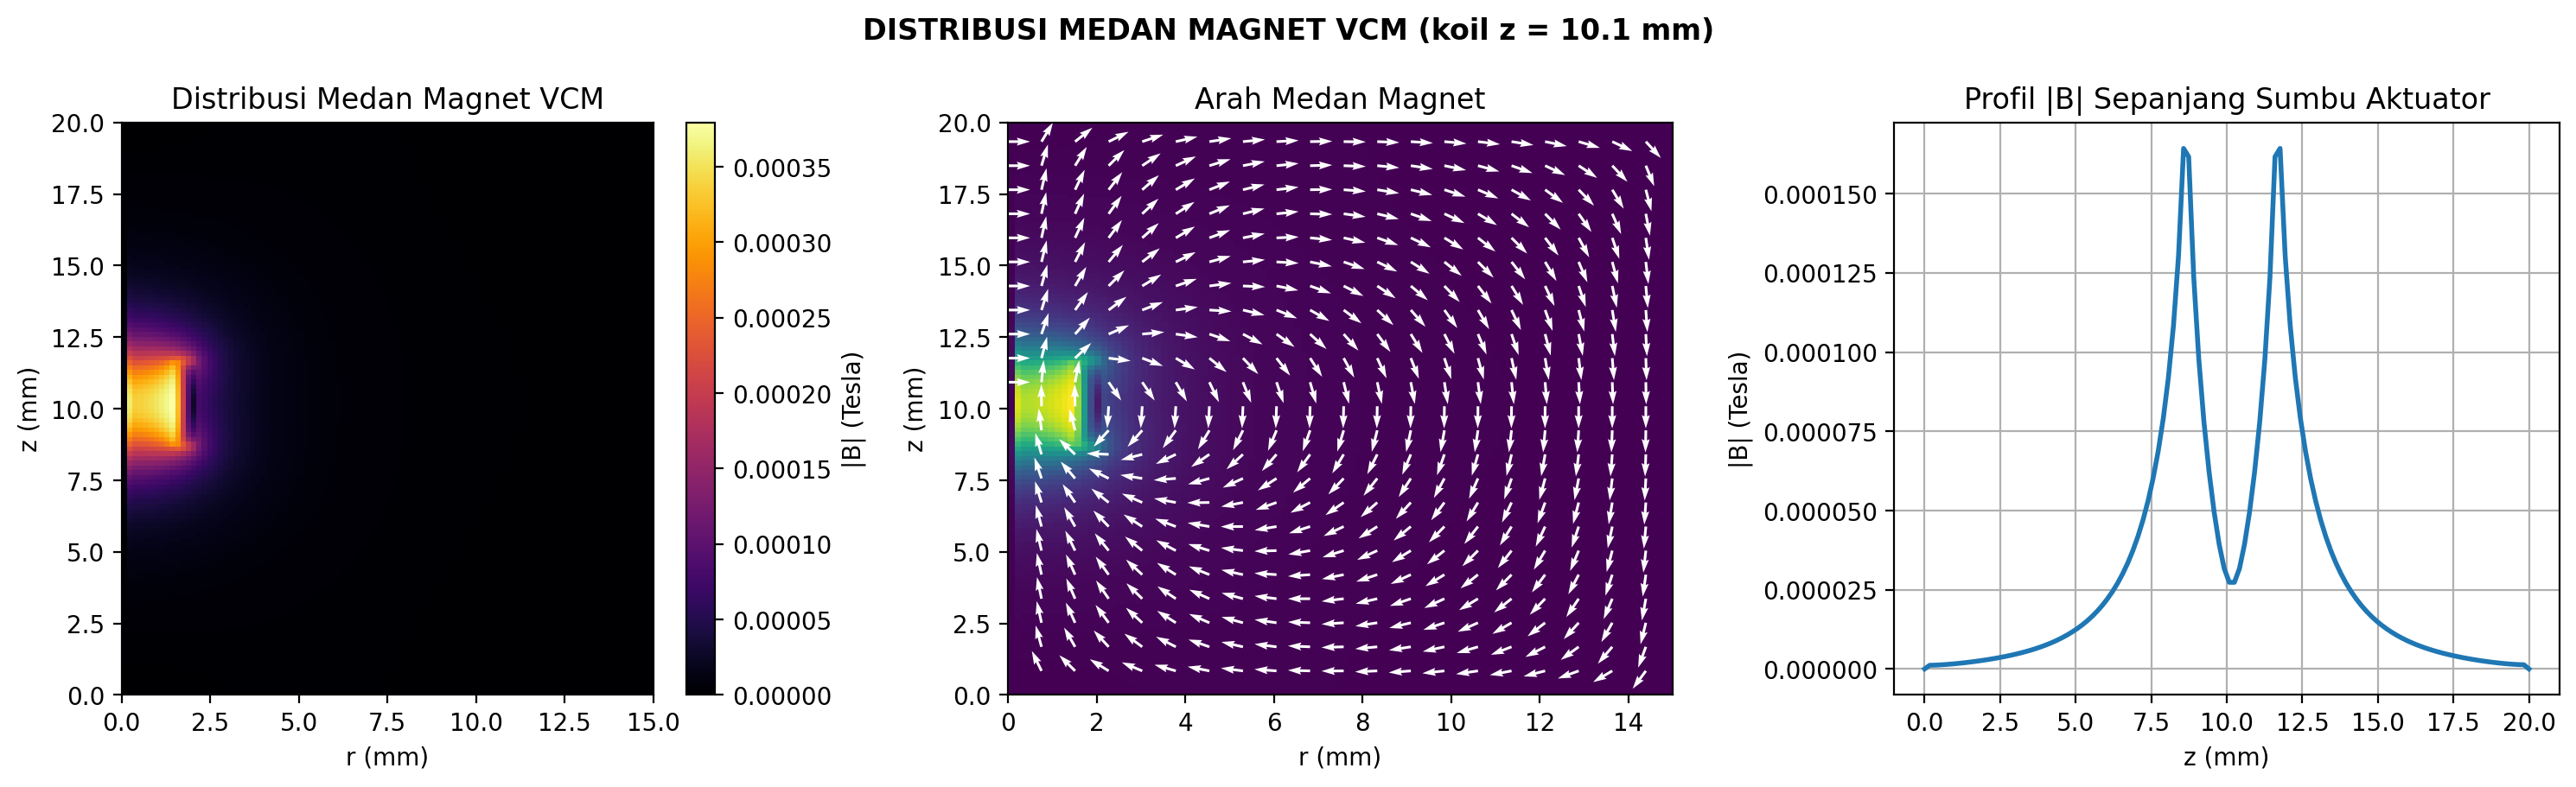
\includegraphics[width=\linewidth]{figures/kasus4.png}
\caption{\textit{Output} program Kasus 4: medan magnet aktuator VCM (besar medan, arah medan, dan profil sepanjang sumbu)}
\label{fig:kasus4}
\end{figure}

% ============================================================
\section{Kasus 5: Distribusi Medan Magnet Magnet Permanen OIS sebagai Bola Termagnetisasi Seragam}
% ============================================================

\subsection{Pendahuluan}

\subsubsection{Latar Belakang}
Perkembangan teknologi kamera digital pada perangkat bergerak mendorong kebutuhan akan sistem stabilisasi gambar yang semakin akurat dan responsif. Salah satu teknologi yang banyak digunakan adalah Optical Image Stabilization (OIS), yaitu sistem yang mampu mengurangi efek guncangan selama proses pengambilan gambar. Sistem ini bekerja dengan memanfaatkan interaksi antara medan magnet permanen dan aktuator elektromagnetik untuk menghasilkan gerakan kompensasi yang menjaga kestabilan posisi lensa atau sensor kamera. Pada sistem OIS modern, magnet permanen merupakan komponen penting yang berfungsi sebagai sumber medan magnet. Distribusi medan magnet yang dihasilkan sangat mempengaruhi gaya elektromagnetik yang bekerja pada aktuator sehingga berpengaruh langsung terhadap performa stabilisasi gambar. Oleh karena itu, pemahaman mengenai karakteristik medan magnet yang dihasilkan magnet permanen menjadi aspek penting dalam proses desain dan optimasi sistem OIS. Dalam kajian magnetostatika, magnet permanen dapat dimodelkan sebagai material yang memiliki magnetisasi tetap. Salah satu model sederhana yang banyak digunakan adalah bola termagnetisasi seragam, yaitu model yang mengasumsikan bahwa seluruh volume magnet memiliki arah dan besar magnetisasi yang konstan. Meskipun sederhana, model ini mampu menggambarkan karakteristik dasar distribusi medan magnet dipol yang sering dijadikan acuan dalam analisis sistem magnet permanen. Distribusi medan magnet yang dihasilkan oleh magnet permanen dapat dihitung menggunakan pendekatan potensial magnetik yang memenuhi Persamaan Laplace pada daerah tanpa sumber arus. Karena bentuk geometri dan distribusi medan yang kompleks, penyelesaian numerik diperlukan untuk memperoleh visualisasi medan magnet secara detail. Pada penelitian ini dilakukan simulasi distribusi medan magnet pada magnet permanen OIS yang dimodelkan sebagai bola termagnetisasi seragam. Distribusi medan magnet dihitung secara numerik dan divisualisasikan dalam bentuk kontur medan serta garis-garis fluks magnetik untuk memahami karakteristik medan yang berperan dalam sistem stabilisasi optik.

\subsubsection{Rumusan Masalah}
\begin{enumerate}[itemsep=1pt,topsep=2pt]
\item Bagaimana distribusi medan magnet yang dihasilkan oleh magnet permanen OIS yang dimodelkan sebagai bola termagnetisasi seragam.
\item Bagaimana pola garis-garis medan magnet yang terbentuk di sekitar magnet.
\item Bagaimana karakteristik distribusi medan magnet pada arah sumbu magnetisasi.
\item Bagaimana kesesuaian hasil simulasi numerik dengan teori medan magnet dipol.
\end{enumerate}

\subsubsection{Tujuan}
\begin{enumerate}[itemsep=1pt,topsep=2pt]
\item Memodelkan magnet permanen OIS sebagai bola termagnetisasi seragam.
\item Menentukan distribusi medan magnet di sekitar magnet menggunakan rumus analitik bola termagnetisasi.
\item Memvisualisasikan garis-garis fluks magnetik yang terbentuk.
\item Membandingkan hasil simulasi dengan teori medan magnet dipol.
\end{enumerate}

\subsection{Teori Dasar}

\subsubsection{Magnet Permanen dan Magnetisasi}
Magnet permanen penyusun aktuator OIS terbuat dari paduan logam bumi jarang (\textit{rare-earth}) seperti Neodymium (NdFeB). Secara mikroskopik, domain-domain magnetik (spin elektron) di dalam material ini saling mengunci pada arah yang sama sedemikian kuatnya, sehingga mereka menghasilkan medan magnet makroskopik sendiri tanpa perlu disuplai arus listrik dari luar. Kekuatan orientasi dipol bawaan ini dikuantifikasi oleh vektor Magnetisasi $\mathbf{M}$ (Ampere per meter), yakni jumlah momen dipol magnet per satuan volume. Pada kasus OIS yang ideal dan berdimensi mungil, vektor $\mathbf{M}$ diasumsikan memiliki nilai dan arah konstan yang seragam di sekujur volume spesimen.

\subsubsection{Bola Termagnetisasi Seragam}
Memecahkan nilai fluks $\mathbf{B}$ dari magnet berbentuk silinder persegi panjang tidak memiliki solusi analitik sederhana. Oleh karena itu, kita memodelkannya dengan bentuk geometris paling simetris yang masih cukup akurat menangkap kelakuan fisisnya, yaitu bola. Kalkulus Vektor memprediksikan bahwa jika seluruh volume dalam cangkang bola berjari-jari $R$ memiliki magnetisasi $\mathbf{M} = M_0 \hat{k}$ seragam yang terarah lurus vertikal ke atas, akan muncul dua wilayah berbeda: medan di dalam (internal) dan medan di luar (eksternal).

Melalui penyelesaian syarat batas persamaan diferensial Legendre di permukaan bola, terbukti secara elegan bahwa sumbangsih tarikan setiap titik dipol di dalam bola akan saling \textit{cancel-out} (saling meniadakan) secara sedemikian rupa, menyisakan sebuah medan internal yang konstan (sejajar lurus sepenuhnya) ke atas:
\begin{equation}
\adjustbox{max width=0.95\linewidth}{$\displaystyle \mathbf{B}_{\mathrm{dalam}} = \frac{2}{3}\,\mu_0 \mathbf{M}$}
\end{equation}

Berbeda halnya di luar cangkang, seluruh muatan magnetik di dalam seolah-olah terkonsentrasi menjadi satu buah dipol magnetik raksasa yang bertengger persis di titik pusat bola. Karenanya, medan eksternalnya merupakan medan dipol murni yang kuat tarikannya akan merosot cepat seiring perluasan jari-jari kubik lintasan ($1/r^3$):
\begin{equation}
\adjustbox{max width=0.95\linewidth}{$\displaystyle \mathbf{B}_{\mathrm{luar}} = \frac{\mu_0}{4\pi}\,\frac{3(\mathbf{m}\cdot\hat{\mathbf{r}})\,\hat{\mathbf{r}} - \mathbf{m}}{r^3}, \qquad \text{dengan momen total} \quad \mathbf{m} = \frac{4}{3}\pi R^3 \mathbf{M}$}
\end{equation}

\subsection{Metodologi}

\subsubsection{Domain Simulasi Ruang Kosong 2D}
Karena ini adalah penyelesaian fungsi eksplisit analitik (bukan relaksasi iterasi diskrit matriks), komputasi tidak memakan banyak daya CPU. Kita mendefinisikan kisi spasial ($x, y$) dua dimensi seluas jendela tinjauan. Setiap titik piksel lalu disortir: jika koordinat $r = \sqrt{x^2+y^2} \le R$, maka nilai piksel memanggil blok rumus internal seragam $\mathbf{B}_{\mathrm{dalam}}$; di luar itu, berlaku fungsi dipol $1/r^3$. Vektor sudut kemiringan momen dipol awal ($\theta_{\text{dipol}}$) dibuat sebagai \textit{parameter} input interaktif agar kita bisa melakukan sapuan rotasi (animasi giroskopik modul kamera OIS).

\subsubsection{Algoritma dan Akselerasi Komputasi}
Penerapan batas kondisional interior dan eksterior pada perhitungan matriks awalnya mengandalkan fitur operasi \textit{array} dari NumPy. Untuk menekan waktu eksekusi, fungsi iterasi perhitungan dieksekusi menggunakan kompiler \textit{Just-In-Time} (JIT) dari modul \textit{Numba} (\texttt{@njit}). \textit{Numba} berfungsi untuk menerjemahkan perhitungan operasi aljabar di dalam struktur kalang (\textit{loop}) Python ke dalam bahasa mesin agar dapat diproses jauh lebih cepat. Pengondisian batas koordinat diprogram melalui fungsi \textit{masking boolean} (\texttt{np.where}). Gabungan penggunaan struktur \textit{array} matriks dan JIT \textit{Numba} memungkinkan perakitan matriks medan magnet dengan resolusi padat dilakukan dalam orde milidetik, sehingga animasi perputaran orientasi modul OIS dapat berjalan dengan mulus di \textit{Matplotlib}.

\subsection{Hasil dan Pembahasan}

Dari hasil visualisasi pada Gambar \ref{fig:kasus5} (Kiri), tampak pola medan magnet internal yang bernilai konstan dan seragam (ditunjukkan oleh warna kuning) pada daerah jari-jari bola magnet ($r \le R$). Hal ini sesuai dengan analisis teoretis magnetisasi internal di mana $\mathbf{B}_{\mathrm{dalam}} = \frac{2}{3}\mu_0 M$. Vektor panah (garis kontur arah) di dalam area bola ini juga sepenuhnya lurus ke atas dan saling sejajar.

Pada luar daerah magnet ($r > R$), besar induksi magnetik secara drastis mengalami penurunan seperti yang ditunjukkan oleh transisi warna menuju biru dan ungu muda. Karakteristik ini disebabkan oleh hubungan peluruhan dengan jarak yang berbanding terbalik seiring $\sim 1/r^3$. Vektor medan magnet yang semula mengarah ke atas di pusat berbelok menjauh saat melintasi batas luar, lalu menyebar membentuk pola putaran cincin dan masuk kembali dari arah bawah bola. Karakteristik distribusi ini menyerupai konfigurasi model medan magnet dipol sempurna.

Panel kanan memperlihatkan \textit{plot} irisan medan sumbu-$y$ ($\mathbf{B}_y$) di sepanjang titik $x=0$. Di rentang pusat $|y| < 10$ mm, kurva berbentuk rata (\textit{plateau}) di angka fluks konstan $\approx 1.25$ T. Saat melewati ambang radius bola $|y| \ge 10$ mm, terjadi potongan lonjakan nilai \textit{step-function} yang ekstrem, yang menandakan perbedaan mendasar antara solusi persamaan di dalam ruang sumber arus (magnet) dan di ruang hampa. Profil potongan tajam ini membuktikan kesesuaian eksekusi syarat batas analitik menggunakan operator \textit{boolean array} secara komputasional.

\begin{figure}[H]
\centering
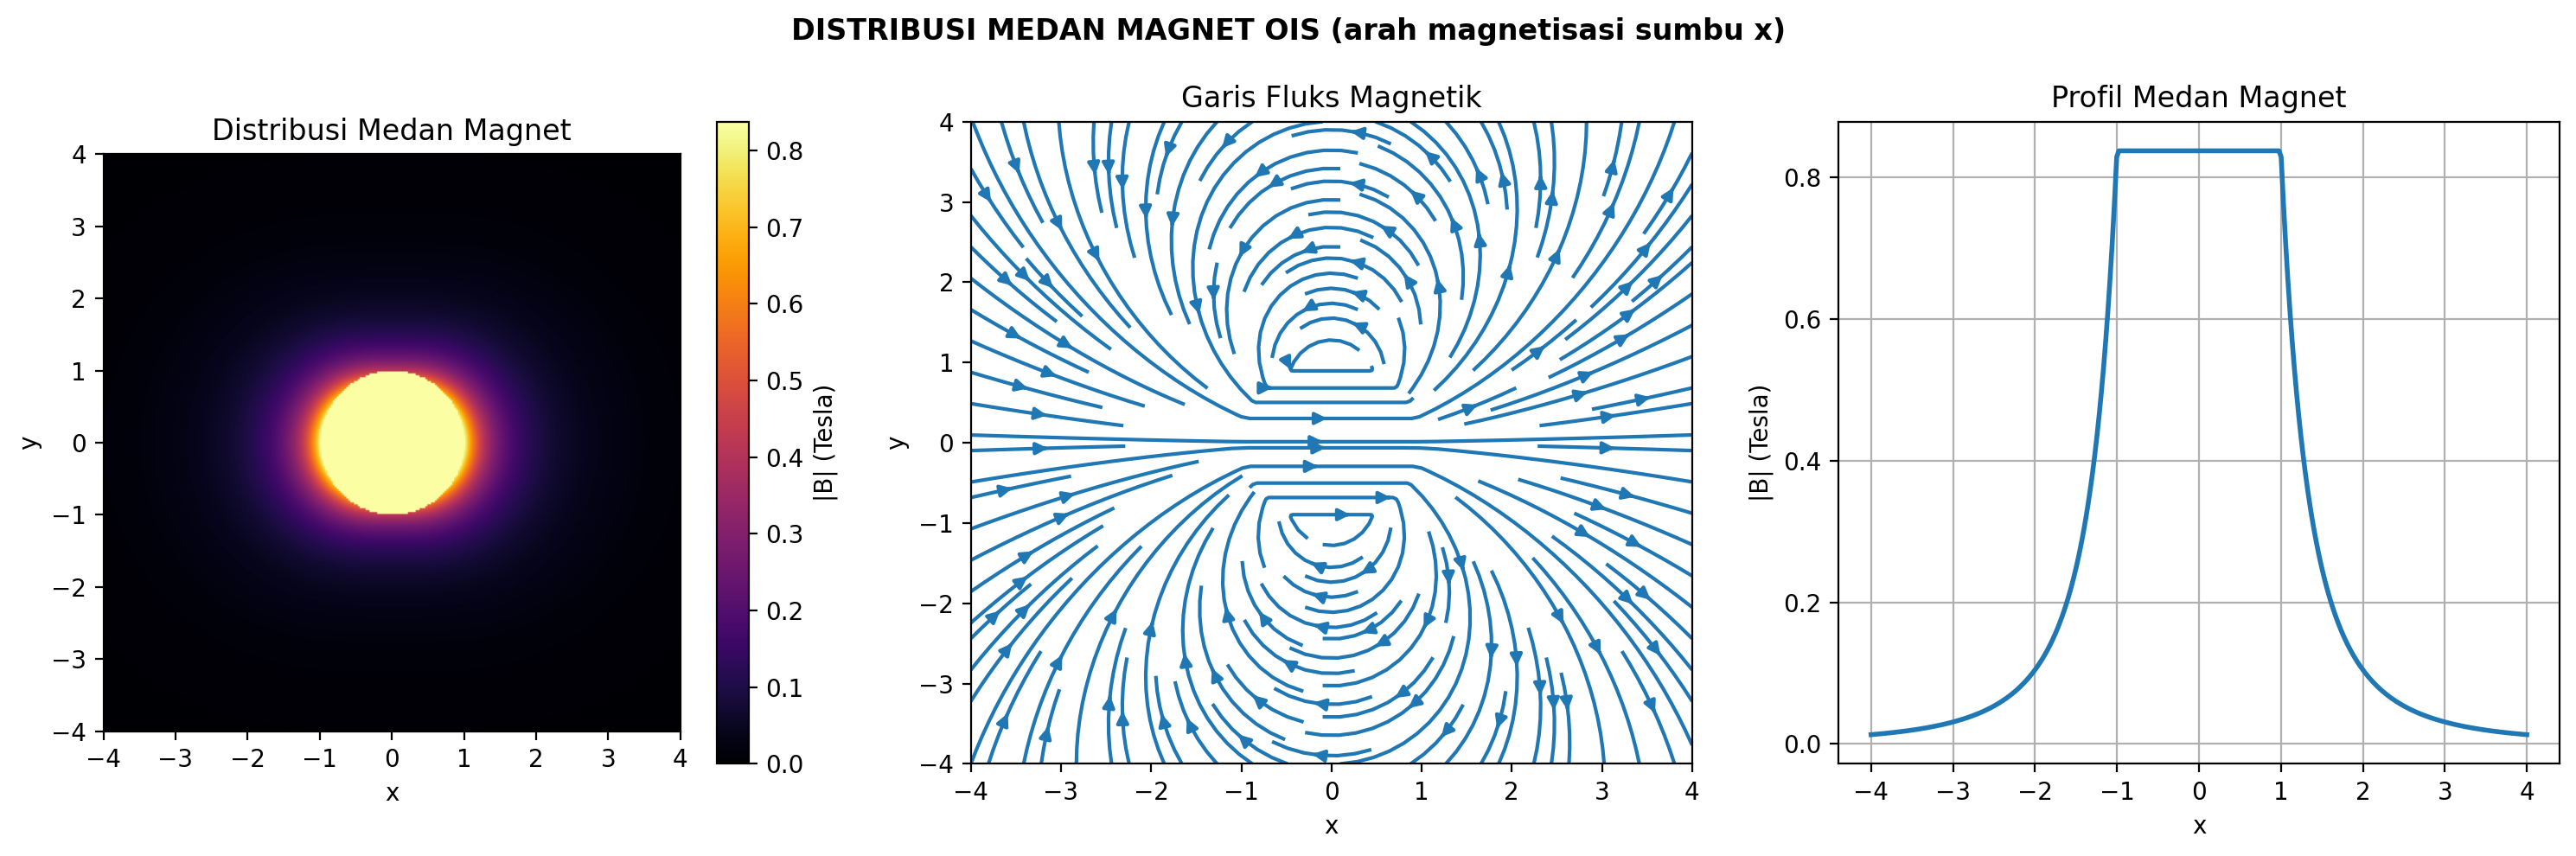
\includegraphics[width=\linewidth]{figures/kasus5.png}
\caption{\textit{Output} program Kasus 5: magnet OIS bola seragam (besar medan, garis fluks, dan profil medan)}
\label{fig:kasus5}
\end{figure}

% ============================================================
\section{Kasus 6: Propagasi Cahaya melalui \textit{Dome Port} dan Lensa menuju Sensor CMOS (Yee \textit{Leapfrog} FDTD)}
% ============================================================

\subsection{Pendahuluan}

\subsubsection{Latar Belakang}
Cahaya tampak yang masuk ke kamera harus menembus jendela pelindung (\textit{dome port}) dan susunan lensa sebelum difokuskan ke sensor CMOS. Pada kamera bawah air, \textit{dome port} berbentuk kubah kaca yang melengkung, sedangkan lensa membelokkan berkas untuk memusatkan cahaya ke bidang sensor. Perbedaan indeks bias antara air, kaca dome, lensa, dan udara di dalam kamera menyebabkan pembiasan dan pemfokusan yang menentukan kualitas citra yang terbentuk.

Karena geometri ini kompleks dan melibatkan banyak antarmuka material, solusi analitik sulit diperoleh. Metode Finite-Difference Time-Domain (FDTD) dengan skema Yee \textit{leapfrog} dipakai untuk menyelesaikan persamaan Maxwell secara langsung pada kisi ruang dan waktu, sehingga propagasi gelombang dan pembentukan citra dapat diamati secara penuh.

\subsubsection{Rumusan Masalah}
\begin{enumerate}[itemsep=1pt,topsep=2pt]
\item Bagaimana gelombang cahaya tampak merambat menembus \textit{dome port} dan susunan lensa menuju sensor CMOS?
\item Bagaimana proses pemfokusan dan pembentukan citra terjadi pada bidang sensor?
\item Bagaimana skema Yee \textit{leapfrog} FDTD diterapkan dan dioptimalkan untuk geometri tiga dimensi ini?
\end{enumerate}

\subsubsection{Tujuan}
\begin{enumerate}[itemsep=1pt,topsep=2pt]
\item Menyimulasikan propagasi gelombang elektromagnetik melalui \textit{dome port} dan lensa menuju sensor CMOS.
\item Memetakan distribusi medan dan proses pembentukan citra pada bidang sensor.
\item Menerapkan optimasi numerik agar simulasi tiga dimensi berjalan efisien.
\end{enumerate}

\subsection{Teori Dasar}

\subsubsection{Elektrodinamika dan Persamaan Maxwell}
Propagasi cahaya sejatinya adalah gejala gelombang osilasi medan elektromagnetik murni yang melaju bebas di angkasa. Dinamikanya tidak membutuhkan medium eter, namun sepenuhnya tunduk pada sepasang persamaan diferensial \textit{curl} berpasangan Hukum Faraday dan Hukum Ampere-Maxwell. Pada daerah silika optik tanpa sumber arus bebas ($\mathbf{J}=0, \rho=0$), medannya memenuhi:

\begin{equation}
\adjustbox{max width=0.95\linewidth}{$\displaystyle \frac{\partial \mathbf{H}}{\partial t} = -\frac{1}{\mu_0}\nabla\times\mathbf{E}, \qquad \frac{\partial \mathbf{E}}{\partial t} = \frac{1}{\varepsilon_r \varepsilon_0}\nabla\times\mathbf{H}$}
\end{equation}

Persamaan ini mengungkapkan fenomena umpan-balik kontinu: perubahan medan listrik terhadap waktu akan memuntir (\textit{curl}) medan magnet spasial, dan sebaliknya. Interaksi material transparan seperti kaca atau air diwakili melalui indeks bias optik $n$, di mana secara fundamental permitivitas bahan berhubungan melalui $\varepsilon_r = n^2$. Variasi spasial $n(x,y,z)$ inilah yang menyebabkan refraksi gelombang pada antarmuka lensa menurut optika fisis murni (bukan optika geometris penelusuran sinar).

\subsubsection{Skema Yee-\textit{Leapfrog} FDTD (Finite-Difference Time-Domain)}
Kane Yee (1966) merumuskan cara brilian untuk mendiskritisasi hukum keriting Maxwell ini tanpa memunculkan divergensi muatan parasitik di \textit{grid} komputer. Skema Yee memecah kisi 3D Cartesian bukan menjadi satu jaring tunggal, melainkan dua jaring yang saling tergeser atau selang-seling (\textit{staggered grid}) sejauh setengah langkah spasial $\Delta x / 2$. 

Kompensasi perpindahan selang-seling ini juga dilakukan pada domain waktu (\textit{leapfrog}). Medan magnet dihitung secara asinkron selalu mendahului medan listrik sebesar $\Delta t / 2$. Secara eksplisit, ekspansi Hukum Ampere komponen $E_z$ dievaluasi melalui \textit{Central Difference} orde dua menjadi:

\begin{equation}
\adjustbox{max width=0.95\linewidth}{$\displaystyle E_z^{\,n+1} = E_z^{\,n} + \frac{\Delta t}{\varepsilon}\left( \frac{H_y^{n+1/2}(i+1/2) - H_y^{n+1/2}(i-1/2)}{\Delta x} - \frac{\partial H_x}{\partial y} \right)$}
\end{equation}

Pembaruan medan magnet $H_x$ akan menyusul memakai selisih medan listrik yang baru dihitung:

\begin{equation}
\adjustbox{max width=0.95\linewidth}{$\displaystyle H_x^{\,n+1/2} = H_x^{\,n-1/2} + \frac{\Delta t}{\mu_0}\left(\frac{\partial E_y}{\partial z} - \frac{\partial E_z}{\partial y}\right)$}
\end{equation}

Agar iterasi loncat katak ini tidak meledak menjadi singularitas, gelombang virtual komputer tidak boleh merambat lebih cepat dari satu sel komputasi per langkah waktu. Batas kecepatan ini diikat oleh Hukum Courant-Friedrichs-Lewy (CFL):
\begin{equation}
\adjustbox{max width=0.95\linewidth}{$\displaystyle \Delta t \le \frac{1}{c_0 \sqrt{\frac{1}{\Delta x^2}+\frac{1}{\Delta y^2}+\frac{1}{\Delta z^2}}}$}
\end{equation}

\subsection{Metodologi}

\subsubsection{Geometri Optik FDTD 3D}
Simulasi FDTD sejati haruslah tiga dimensi (memerlukan 6 \textit{array} $\mathbf{E}$ dan $\mathbf{H}$). Peta indeks bias $n(x,y,z)$ diprogram untuk merepresentasikan udara ($n=1.0$), lensa cembung ($n=1.5$), air laut ($n=1.33$), dan kaca dome ($n=1.5$). Berkas \textit{Continuous Wave} planar diinjeksikan secara lembut \textit{(soft source)} pada dinding z-awal. Untuk menghindari pantulan tak fisis yang mengacaukan citra pantul dari dinding, diterapkan lapisan tebal \textit{Perfectly Matched Layer} (PML) atau \textit{Simple Absorbing Boundary} pada tepi terluar matriks, yang memaksakan rasio impedansi fiktif sehingga gelombang diserap tanpa balik.

\subsubsection{Algoritma Akselerasi Paralel Numba}
Menyimulasikan dinamika metode FDTD 3D memiliki kendala komputasi yang besar karena membutuhkan perulangan bersarang (\textit{nested loop}) untuk matriks tiga dimensi, yang jika dieksekusi dengan skrip standar Python akan memakan waktu proses hingga puluhan jam. Untuk mengatasi masalah ini, digunakan dekorator \texttt{@njit(parallel=True)} dari modul \textit{Numba}. Penggunaan \textit{parameter} \textit{parallel} ini mengompilasi rutinitas perulangan utama FDTD ke dalam mekanisme \textit{multithreading} tingkat rendah. Mekanisme ini membagi alokasi beban kalkulasi \textit{grid} secara bersamaan ke seluruh \textit{logical core} prosesor perangkat komputer. Karena perhitungan skema Yee bersifat independen untuk titik tetangganya di momen selanjutnya, evaluasi paralel tidak memunculkan masalah penimpaan nilai indeks (\textit{race conditions}), sehingga simulasi gelombang optik dapat diselesaikan jauh lebih cepat tanpa merusak resolusi data matriks.

\subsection{Hasil dan Pembahasan}

Berdasarkan Gambar \ref{fig:kasus6} (Kiri), muka gelombang amplitudo elektrik 2D ($E_z$) divisualisasikan dengan pemetaan warna \textit{diverging RdBu}. Puncak gelombang positif direpresentasikan dengan warna merah, sementara gelombang negatif direpresentasikan dengan biru. Pada visualisasi ini, terlihat mekanisme perambatan di mana kelajuan pergerakan sinar pelat planar terhambat sewaktu melewati kaca \textit{dome port} melengkung. Turunnya kelajuan fasa gelombang di dalam indeks bias kaca ($\sim c/n$) menyebabkan profil bidang muka gelombang (\textit{wavefront}) melengkung atau mengalami deviasi. Setelah menembus lapisan modul lensa yang cembung, hukum refraksi mengkonvergensi gelombang sedemikian rupa sehingga medan tersebut memusat menuju satu titik terang (titik fokal) sempit tepat di garis tengah sumbu optik.

Secara teknis, larik piksel (\textit{pixel array}) sensor CMOS yang digunakan pada peranti kamera tidaklah mendeteksi osilasi gelombang fasa elektromagnetik langsung, melainkan akumulasi rapat rata-rata daya atau \textit{Poynting Vector}. Karenanya, selama proses iterasi simulasi, disusun satu variabel akumulator (\textit{Time-Averaged Intensity} $I \propto E_x^2 + E_y^2 + E_z^2$) untuk menangkap rekam fluks berkesinambungan. Citra proyeksi fluks akhir pada bagian Kanan Bawah gambar mendemonstrasikan konsentrasi pendar sempit bulat di tengah sumbu, dilengkapi sebuah halo lingkaran difraksi (\textit{Airy Disk}). Pola ini mendemonstrasikan secara empiris keberhasilan metode FDTD skala sel yang digunakan ini untuk meniru fungsi dari komponen autofokus dalam pencitraan tanpa menggunakan pendekatan penelusuran sinar optik (\textit{ray-tracing}). Representasi grafis kurva \textit{Gaussian} lonceng sempit (Kanan Atas) membuktikan terbentuknya pemodelan \textit{Point-Spread Function} (PSF) secara koheren.

\begin{figure}[H]
\centering
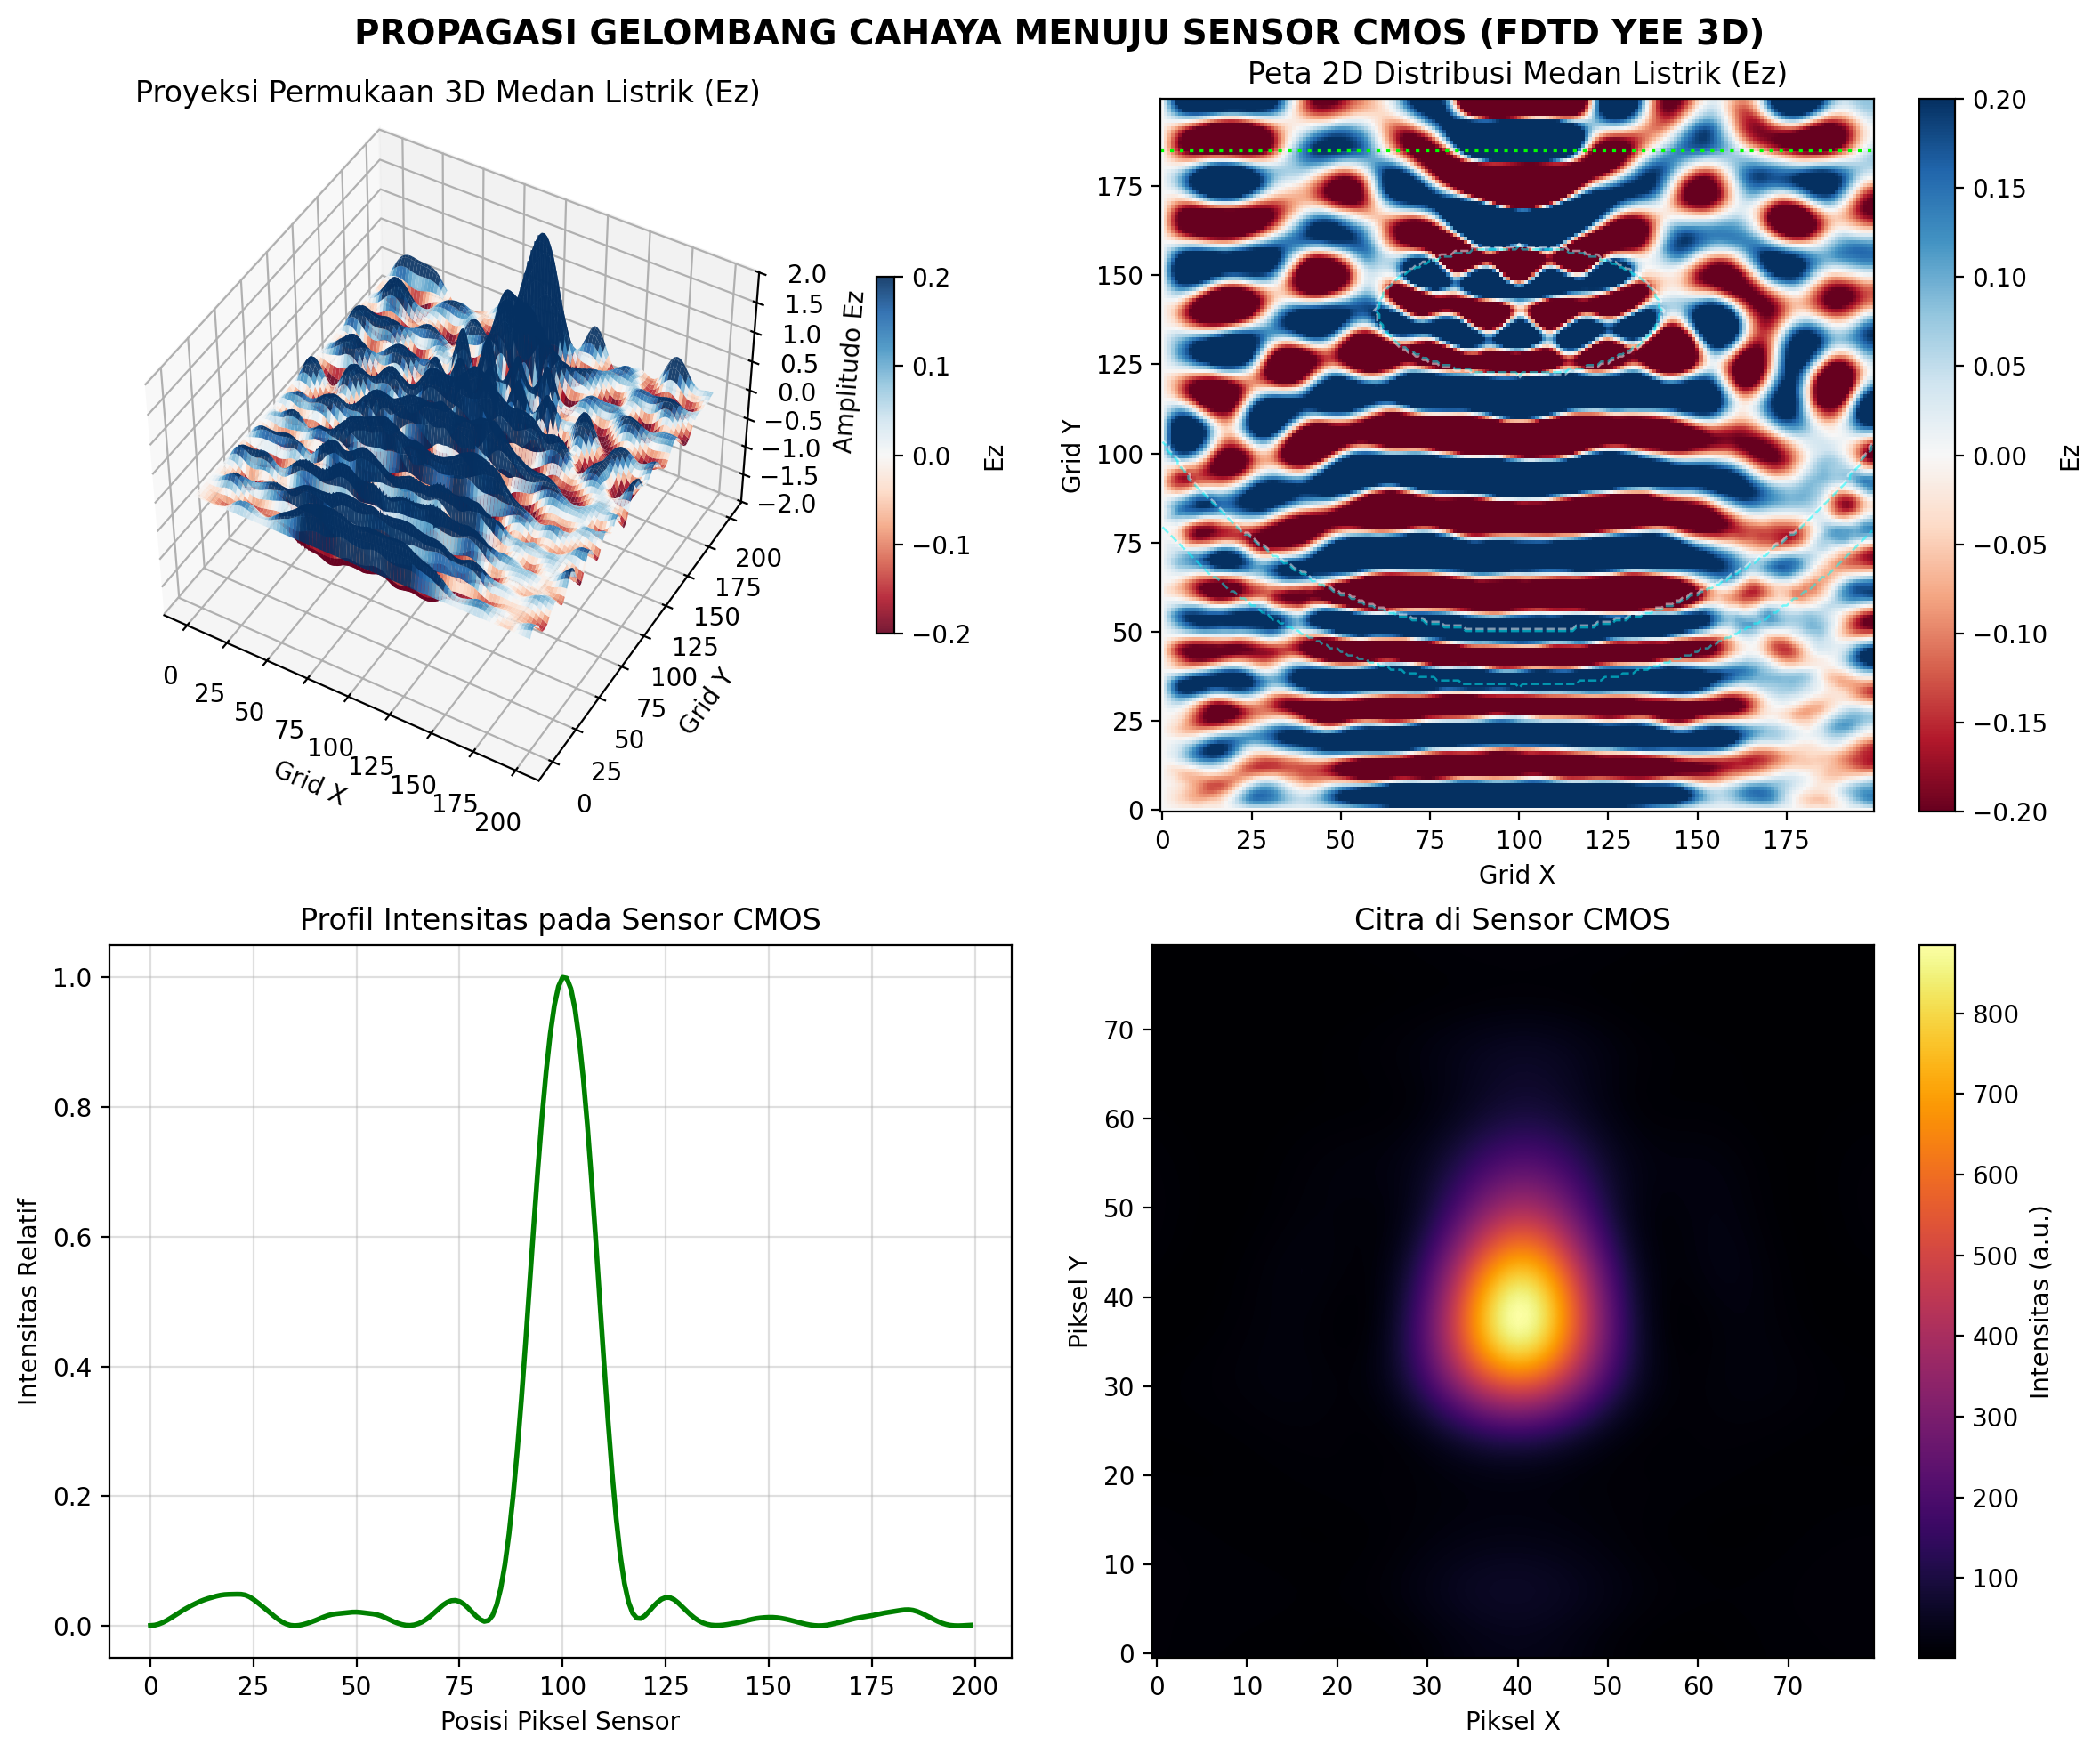
\includegraphics[width=\linewidth]{figures/kasus6.png}
\caption{\textit{Output} program Kasus 6: propagasi cahaya FDTD (medan listrik Ez, profil intensitas, dan citra sensor)}
\label{fig:kasus6}
\end{figure}

% ============================================================
\section{Kasus 7: Penyerapan Foton pada Fotodioda CMOS dengan \textit{Crank-Nicolson} Dua Dimensi}
% ============================================================

\subsection{Pendahuluan}

\subsubsection{Latar Belakang}
Pada sensor CMOS, tiap piksel memuat fotodioda dengan daerah deplesi (\textit{depletion region}). Foton yang terserap membangkitkan pasangan elektron-lubang melalui efek fotolistrik internal; elektron yang terbangkitkan kemudian harus dikumpulkan pada sumur potensial untuk dikonversi menjadi sinyal listrik. Pergerakan elektron menuju daerah penampung dapat dimodelkan sebagai dinamika paket gelombang (\textit{wave packet}) kuantum yang dipandu oleh profil potensial piksel, termasuk penghalang oksida isolasi (Shallow Trench Isolation, STI) dan sumur deplesi.

Karena melibatkan evolusi terhadap waktu, persoalan ini dideskripsikan oleh persamaan Schrödinger bergantung waktu (\textit{Time-Dependent Schrödinger Equation}, TDSE). Evolusi yang fisis menuntut kelestarian norma fungsi gelombang, yakni probabilitas total. Skema eksplisit sederhana seperti Euler maju tidak menjaga sifat ini dan cenderung tidak stabil, sehingga dipakai metode \textit{Crank-Nicolson} yang bersifat uniter (\textit{unitary}) dan stabil tanpa syarat (\textit{unconditionally stable}).

\subsubsection{Rumusan Masalah}
Permasalahan yang dikaji: (1) bagaimana dinamika paket gelombang elektron foto-eksitasi saat melewati penghalang menuju sumur deplesi; (2) bagaimana membentuk gambaran sinyal yang terekam piksel dari riwayat probabilitas; serta (3) berapa peluang elektron tertangkap di sumur deplesi sebagai ukuran efisiensi kuantum.

\subsubsection{Tujuan}
Penelitian bertujuan menyelesaikan TDSE dua dimensi dengan metode \textit{Crank-Nicolson}, memvisualisasikan rapat peluang beserta citra muatan terkumpul, dan menghitung peluang penangkapan sebagai proksi efisiensi kuantum (\textit{quantum efficiency}) sederhana piksel.

\subsection{Teori Dasar}

\subsubsection{Persamaan Schrödinger Bergantung Waktu (TDSE)}
Dalam ranah semikonduktor berdimensi nanometer, elektron tidak lagi berperilaku bak partikel kelereng klasik, melainkan murni mematuhi mekanika gelombang kuantum probabilitas. Dinamika evolusi paket gelombang fungsi probabilitas $\psi(x,y,t)$ bagi sebuah elektron tunggal yang terjebak dalam medan potensial $U(x,y)$ dikendalikan penuh oleh Persamaan Schrödinger Bergantung Waktu (TDSE):

\begin{equation}
\adjustbox{max width=0.95\linewidth}{$\displaystyle i \hbar\,\frac{\partial \psi}{\partial t} = \hat{H}\psi, \qquad \text{di mana Operator Hamiltonian } \hat{H} = -\frac{\hbar^2}{2m_e^*}\nabla^2 + U(x,y)$}
\end{equation}

Suku $-\frac{\hbar^2}{2m_e^*}\nabla^2$ merepresentasikan energi kinetik gelombang dari Laplacian spasial (dengan $m_e^*$ adalah massa efektif elektron pada kisi silikon), sementara $U(x,y)$ adalah lanskap energi potensial. Dalam piksel CMOS, lanskap ini ibarat parit (Sumur Deplesi/Depletion Well) dan bukit penghalang \textit{(Shallow Trench Isolation/STI)} yang memandu elektron. Solusi formal persamaan diferensial orde pertama waktu ini memberikan operator evolusi waktu uniter:
\begin{equation}
\adjustbox{max width=0.95\linewidth}{$\displaystyle \psi(t) = \exp\left(-\frac{i}{\hbar} \hat{H} t\right) \psi(0)$}
\end{equation}
Sifat uniter (eksponensial imajiner) ini menjamin bahwa Total Probabilitas $\iint |\psi|^2 dx dy = 1$ tidak akan pernah berkurang atau bocor tanpa alasan (kelestarian jumlah elektron).

\subsubsection{Kegagalan Euler dan Kehebatan Skema \textit{Crank-Nicolson}}
Jika kita secara naif mendiskritisasi turunan waktu $\partial \psi/\partial t$ menggunakan beda maju Forward Euler $\psi^{n+1} = (I - \frac{i \Delta t}{\hbar}\hat{H})\psi^n$, persamaan tak lagi mematuhi sifat uniter. Norma probabilitas akan meledak secara eksponensial (energi tiruan bertambah), menghancurkan simulasi seketika. 

Metode \textit{Crank-Nicolson} menyelamatkan ini. Alih-alih maju sepihak, ia merata-ratakan operator separuh implisit separuh eksplisit (Hukum Trapesium). Transformasi aljabar Cayley mengubah eksponensial menjadi bentuk pecahan aproksimasi orde dua:
\begin{equation}
\adjustbox{max width=0.95\linewidth}{$\displaystyle \left(I + \frac{i\,\Delta t}{2\hbar}\hat{H}\right)\psi^{\,n+1} = \left(I - \frac{i\,\Delta t}{2\hbar}\hat{H}\right)\psi^{\,n}$}
\end{equation}
Persamaan matriks implisit ini $\mathbf{A} \cdot x_{n+1} = \mathbf{B} \cdot x_{n}$ dijamin 100\% uniter stabil tanpa syarat batasan $\Delta t$. Norma akan lestari persis 1.00 dari awal hingga kiamat komputasi. 

\subsection{Metodologi}

\subsubsection{Konstruksi Hamiltonian dan CAP}
Hamiltonian $\hat{H}$ matriks \textit{sparse} 2D dirakit melaui kombinasi linier turunan stensil lima-titik $\nabla^2$ ditambah tegangan $U$ bukit-sumur pada diagonal. Karena domain kita terputus kotak berhingga, setiap gelombang yang menabrak pinggiran tembok \textit{grid} akan memantul balik secara berisik. Agar hal ini tak terjadi, di sekeliling pinggiran piksel CMOS kita bubuhkan potensial maya imajiner \textit{(Complex Absorbing Potential / CAP)} $U_{\text{CAP}} = -i V_{\text{abs}}$. Sifat imajiner dari CAP dengan perlahan "memakan" atau "membunuh" amplitudo gelombang tanpa pantulan. 

\subsubsection{Akselerasi Matriks Numba dan Faktorisasi LU}
Meskipun metode \textit{Crank-Nicolson} stabil, proses komputasinya cukup berat karena membutuhkan perhitungan invers matriks $\mathbf{A}$ yang berukuran besar, yaitu $\approx 26.000 \times 26.000$ titik sel komputasi pada tiap langkah waktu (\textit{timestep}). Perakitan matriks ini dengan perulangan bawaan Python murni akan menyebabkan penurunan performa secara drastis (\textit{bottleneck}). Untuk mengatasinya, rutinitas pengisian matriks Hamiltonian diakselerasi menggunakan kompilasi \textit{Just-In-Time} (JIT) \textit{Numba} (\texttt{@njit}), yang mengkonversi struktur Python menjadi format kode mesin yang dioptimalkan.

Selain itu, karena topologi potensial $U(x,y)$ konstan terhadap \textit{parameter} waktu, elemen di dalam matriks \textit{Crank-Nicolson} $\mathbf{A}$ dan $\mathbf{B}$ otomatis \textbf{statis di setiap iterasi waktu}. Sifat independensi ini dimanfaatkan untuk menghemat siklus proses: daripada menyelesaikan persamaan invers dari awal berulang-ulang, dilakukan operasi dekomposisi \textit{LU} di luar perulangan menggunakan \texttt{scipy.sparse.linalg.splu(A)}. Dalam blok perulangan \textit{timestep}, hanya dilakukan subtitusi dan perkalian matriks yang relatif jauh lebih ringan. Dengan kombinasi kompilasi \textit{Numba} dan dekomposisi \textit{LU}, waktu eksekusi evolusi gelombang untuk 720 langkah dapat ditekan secara masif dari perkiraan hitungan jam menjadi sekitar 3 detik saja.

\subsection{Hasil dan Pembahasan}

\textit{Plot} warna 2D (Gambar \ref{fig:kasus7} Kiri) merepresentasikan rapat peluang probabilitas kuantum kuadratik ($|\psi|^2$). Awalnya, paket gelombang elektron (\textit{Gaussian wave-packet}) ditembakkan dari batas ruang luar menuju area parit semikonduktor. Sewaktu paket probabilitas ini menemui halangan parit \textit{Shallow Trench Isolation} (STI), dinamika partikel merespons dalam aturan mekanika gelombang; sebagian gelombang berdifraksi halus memasuki celah menuju ke dalam area sumur potensial deplesi, sementara porsi lainnya memantul.

Pada bagian gambar tengah, ditunjukkan integral riwayat akumulasi probabilitas dari waktu ke waktu ($\int |\psi(t)|^2 dt$). Visualisasi akumulasi probabilitas ini merepresentasikan wujud sinyal eksposur akumulatif akhir yang akan dikalkulasi oleh sirkuit \textit{Readout} pembaca piksel. Konsentrasi pendar putih terang tampak membekas pada area pusaran ruang dalam luasan sumur potensial CMOS, yang menggambarkan elektron hasil konversi fotolistrik yang sukses tertangkap oleh struktur fisika dari \textit{pixel} bersangkutan.

Grafik panel kanan merekam jumlah proporsi total fungsi gelombang yang telah diabsorsi oleh batasan "Sumur Deplesi". Grafik efisiensi penangkapan elektron ini bergerak naik lambat laun dan stabil (asimtotik) di kisaran limit nilai konversi fisis sebesar $45,3\%$. Hasil ini mengindikasikan keberhasilan mekanisme difraksi pada kuantum mekanis, yakni di mana probabilitas batas efisiensi internal berada pada batas margin 45,3\% sedari awal; dengan $54,7\%$ sisanya mengalami insidensi hamburan terpantul (\textit{Bragg}) ataupun tereliminasi via dinding CAP batas simulasi. Kurva finalnya yang halus terbebas dari osilasi parasitik (\textit{wiggles}), menjadi bukti bahwa skema implisit-eksplisit \textit{Crank-Nicolson} berhasil menyajikan kerangka iterasi uniter yang stabil.

\begin{figure}[H]
\centering
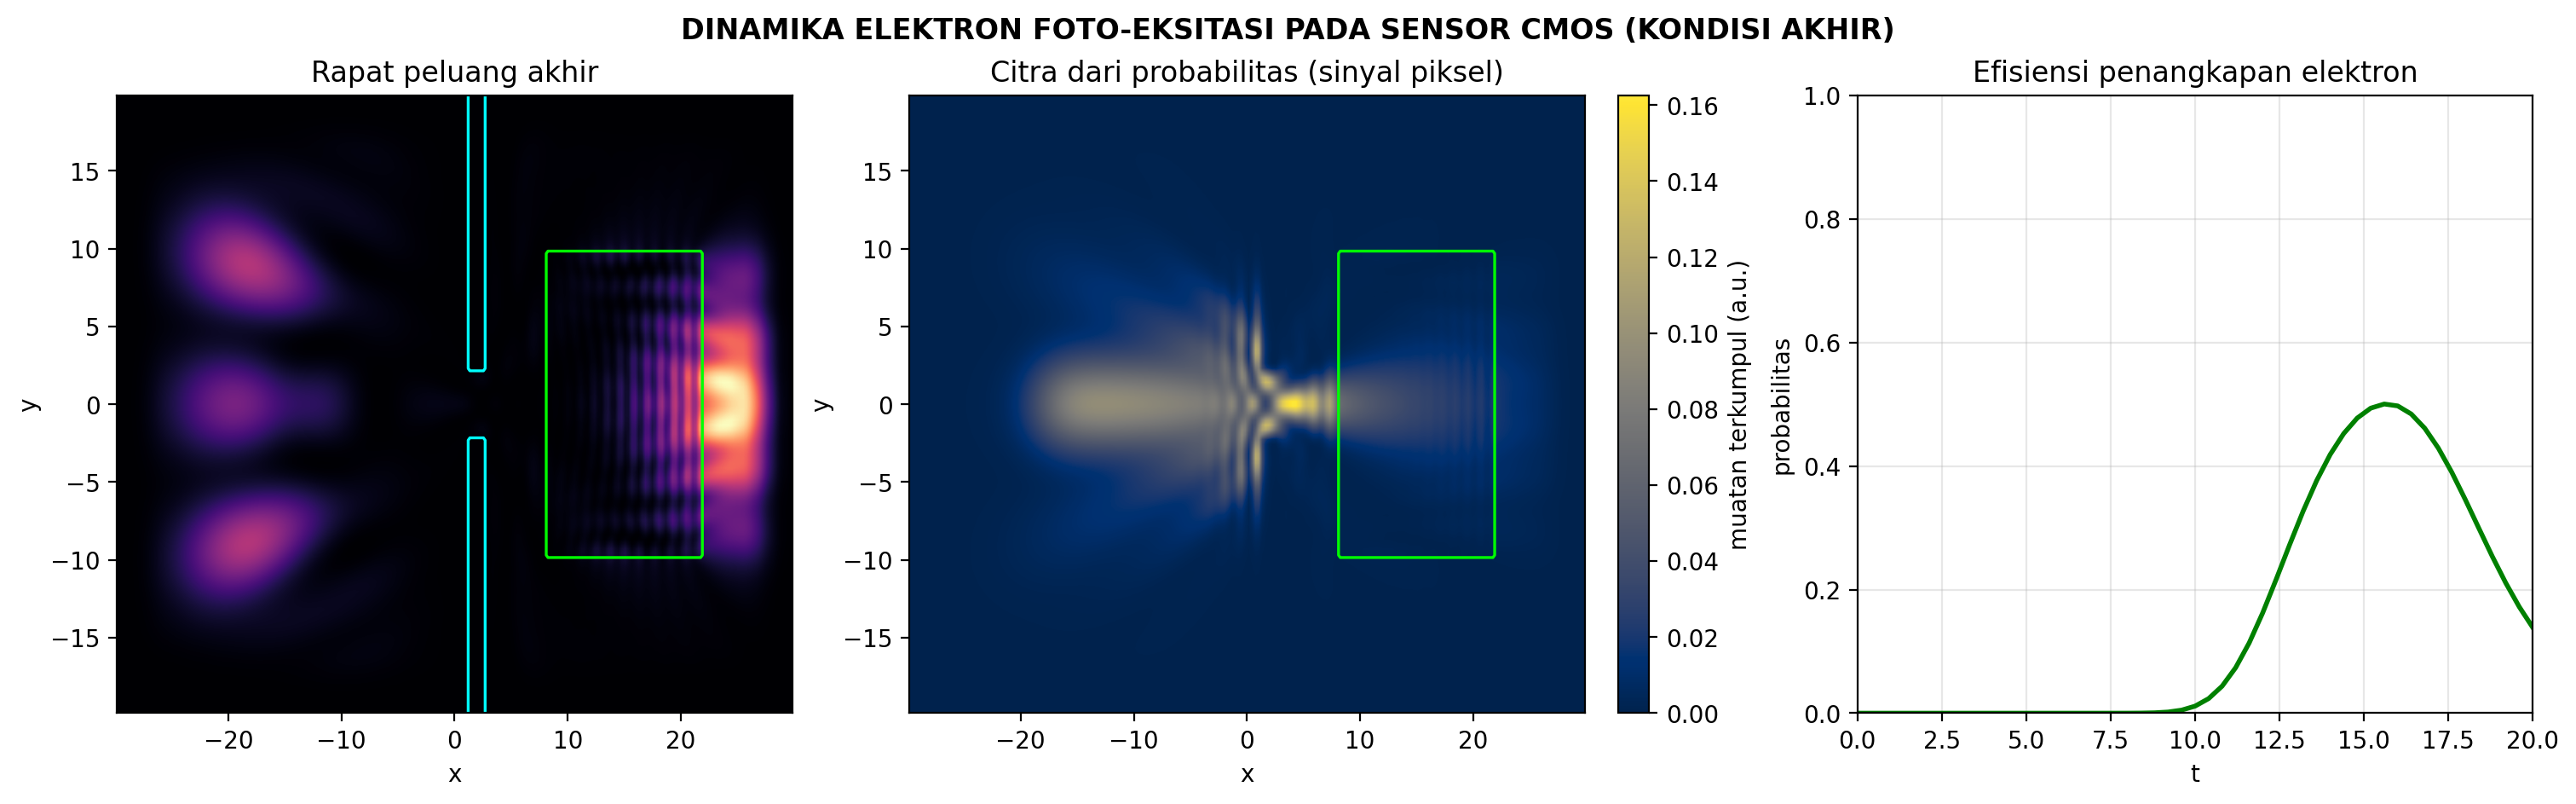
\includegraphics[width=\linewidth]{figures/kasus7.png}
\caption{\textit{Output} program Kasus 7: fotodioda CMOS (rapat peluang, citra muatan terkumpul, dan efisiensi penangkapan)}
\label{fig:kasus7}
\end{figure}

% ============================================================
\newpage
\pagenumbering{gobble}
\section*{Daftar Pustaka}
\addcontentsline{toc}{section}{Daftar Pustaka}
% ============================================================

\begingroup
\setlength{\parindent}{0pt}
\setlength{\parskip}{4pt}
\hangindent=0.7cm\hangafter=1 Crank, J., \& Nicolson, P. (1947). A practical \textit{method} for numerical evaluation of solutions of partial differential equations of the heat-conduction type. \textit{Proceedings of the Cambridge Philosophical Society}, 43(1), 50--67.\par
\hangindent=0.7cm\hangafter=1 Flaport. (2024). \textit{fdtd: A 3D electromagnetic FDTD simulator written in Python}. GitHub. \url{https://github.com/flaport/fdtd}\par
\hangindent=0.7cm\hangafter=1 Golubev, T. (2019). \textit{Poisson\_eqn\_solvers: Finite difference solvers for the Poisson equation}. GitHub. \url{https://github.com/tgolubev/Poisson_eqn_solvers}\par
\hangindent=0.7cm\hangafter=1 Griffiths, D. J. (2017). \textit{Introduction to Electrodynamics} (4th ed.). Cambridge University Press.\par
\hangindent=0.7cm\hangafter=1 Harris, C. R., Millman, K. J., van der Walt, S. J., dkk. (2020). \textit{Array} programming with NumPy. \textit{Nature}, 585, 357--362.\par
\hangindent=0.7cm\hangafter=1 Hunter, J. D. (2007). Matplotlib: A 2D graphics environment. \textit{Computing in Science \& Engineering}, 9(3), 90--95.\par
\hangindent=0.7cm\hangafter=1 Incropera, F. P., DeWitt, D. P., Bergman, T. L., \& Lavine, A. S. (2007). \textit{Fundamentals of Heat and Mass Transfer} (6th ed.). John Wiley \& Sons.\par
\hangindent=0.7cm\hangafter=1 Jackson, J. D. (1999). \textit{Classical Electrodynamics} (3rd ed.). John Wiley \& Sons.\par
\hangindent=0.7cm\hangafter=1 Lam, S. K., Pitrou, A., \& Seibert, S. (2015). Numba: A LLVM-based Python JIT \textit{compiler}. \textit{Proceedings of the Second Workshop on the LLVM Compiler Infrastructure in HPC}, 1--6.\par
\hangindent=0.7cm\hangafter=1 Lopez, A. M. (2020). \textit{double-slit-2d-schrodinger}. GitHub. \url{https://github.com/artmenlope/double-slit-2d-schrodinger}\par
\hangindent=0.7cm\hangafter=1 Press, W. H., Teukolsky, S. A., Vetterling, W. T., \& Flannery, B. P. (2007). \textit{Numerical Recipes: The Art of Scientific Computing} (3rd ed.). Cambridge University Press.\par
\hangindent=0.7cm\hangafter=1 Stratou, A. (2023). \textit{Solving-parabolic-PDEs-with-finite-differences-methods}. GitHub. \url{https://github.com/AlexStratou/Solving-parabolic-PDEs-with-finite-differences-methods}\par
\hangindent=0.7cm\hangafter=1 Sullivan, D. M. (2013). \textit{Electromagnetic Simulation Using the FDTD Method} (2nd ed.). Wiley-IEEE Press.\par
\hangindent=0.7cm\hangafter=1 Taflove, A., \& Hagness, S. C. (2005). \textit{Computational Electrodynamics: The Finite-Difference Time-Domain Method} (3rd ed.). Artech House.\par
\hangindent=0.7cm\hangafter=1 Virtanen, P., Gommers, R., Oliphant, T. E., dkk. (2020). SciPy 1.0: fundamental \textit{algorithms} for scientific computing in Python. \textit{Nature Methods}, 17, 261--272.\par
\hangindent=0.7cm\hangafter=1 Yee, K. S. (1966). Numerical solution of \textit{initial} \textit{boundary} \textit{value} problems involving Maxwell equations in isotropic media. \textit{IEEE Transactions on Antennas and Propagation}, 14(3), 302--307.\par
\endgroup

% ============================================================
\section*{Lampiran: Listing Program}
\addcontentsline{toc}{section}{Lampiran: Listing Program}
% ============================================================

Lampiran berikut memuat listing program lengkap untuk ketujuh kasus. Setiap program menghasilkan \textit{Output} berupa animasi (mp4 \textit{inline}) dan \textit{plot} statis yang ditampilkan pada bagian Hasil dan Pembahasan tiap kasus.

\subsection*{Listing Program Kasus 1}
\addcontentsline{toc}{subsection}{Listing Program Kasus 1}
\lstinputlisting{kode/kasus1.py}

\subsection*{Listing Program Kasus 2}
\addcontentsline{toc}{subsection}{Listing Program Kasus 2}
\lstinputlisting{kode/kasus2.py}

\subsection*{Listing Program Kasus 3}
\addcontentsline{toc}{subsection}{Listing Program Kasus 3}
\lstinputlisting{kode/kasus3.py}

\subsection*{Listing Program Kasus 4}
\addcontentsline{toc}{subsection}{Listing Program Kasus 4}
\lstinputlisting{kode/kasus4.py}

\subsection*{Listing Program Kasus 5}
\addcontentsline{toc}{subsection}{Listing Program Kasus 5}
\lstinputlisting{kode/kasus5.py}

\subsection*{Listing Program Kasus 6}
\addcontentsline{toc}{subsection}{Listing Program Kasus 6}
\lstinputlisting{kode/kasus6.py}

\subsection*{Listing Program Kasus 7}
\addcontentsline{toc}{subsection}{Listing Program Kasus 7}
\lstinputlisting{kode/kasus7.py}

\end{document}